\documentclass{rapportENSIAS}
\definecolor{bg}{rgb}{0.95,0.95,0.95}

\usepackage{titlesec}
\usepackage{tocloft}
\usepackage{booktabs}
\usepackage{tabularx}
\usepackage{float}
\usepackage{enumitem}
\usepackage{longtable}
\usepackage{setspace}

% TikZ et bibliothèques
\usepackage{tikz}
\usetikzlibrary{positioning,shadows,fit,shapes.geometric,arrows.meta,calc,backgrounds}
\definecolor{bmcblue}{HTML}{DCEEFF}
\definecolor{bmcaccent}{HTML}{1F4FD8}

% Couleurs du projet
\definecolor{rougeENSIAS}{RGB}{180,30,30}
\definecolor{bleuUM5}{RGB}{0,80,160}
\definecolor{grisfonce}{RGB}{50,50,50}
\definecolor{orangecode}{RGB}{230,126,34}
\definecolor{vertcode}{RGB}{0,128,0}

% Commande pour les emplacements de captures d'écran
% Usage: \screenshot[largeur]{Description de la capture}
\newcommand{\screenshot}[2][\textwidth]{%
  \begin{figure}[H]
    \centering
    \fbox{\parbox{#1}{\vspace{4cm}\centerline{\textit{\large #2}}\vspace{4cm}}}
  \end{figure}
}

\title{Rapport PFA -- SmartBI}

\begin{document}

%----------- Informations du rapport ---------

\titre{Plateforme de Business Intelligence pilotée par des agents d'Intelligence Artificielle utilisant LangGraph et des modèles de langage locaux}
\sujet{Projet de Fin d'Année -- Business Intelligence \& Analytics}

\enseignant{ \textsc{ Pr Y. ALAMI   }}

\eleves{Salah Eddine \textsc{ABBASSI} \\ Selimane \textsc{Ait Si Elmadani} }

\jury{\textsc{ Pr. .....} \\ \textsc{ Pr. ....}}

%----------- Initialisation -------------------

\fairemarges
\fairepagedegarde
\chapter*{Dédicaces}
\addcontentsline{toc}{chapter}{Dédicaces}

Nous dédions ce modeste travail à nos parents, dont le soutien inconditionnel et les sacrifices ont rendu possible notre parcours académique. À nos familles et à tous ceux qui nous ont soutenus, encouragés et inspirés tout au long de notre formation à l'ENSIAS.

\chapter*{Remerciements}
\addcontentsline{toc}{chapter}{Remerciements}

Nous tenons tout d'abord à exprimer nos sincères remerciements à notre encadrant, le Professeur Y.~ALAMI, pour sa disponibilité, ses conseils avisés et son accompagnement tout au long de la réalisation de ce projet. Son expertise dans le domaine de l'informatique décisionnelle et de l'intelligence artificielle a été déterminante dans l'orientation de nos travaux.

Nous remercions également l'ensemble du corps professoral de l'École Nationale Supérieure d'Informatique et d'Analyse des Systèmes (ENSIAS) pour la qualité de la formation dispensée durant notre cursus d'ingénieur, qui nous a fourni les bases théoriques et pratiques nécessaires à la conduite de ce projet.

Nous adressons nos remerciements à nos collègues et camarades de promotion pour leurs retours constructifs et l'entraide mutuelle tout au long de l'année universitaire.

Enfin, nous remercions les membres du jury pour l'intérêt qu'ils portent à ce travail en acceptant de l'évaluer.

%==============================================================================
% RÉSUMÉS
%==============================================================================
\chapter*{Résumé}
\addcontentsline{toc}{chapter}{Résumé}

Dans un contexte où les données constituent un actif stratégique majeur pour les entreprises, leur exploitation efficace demeure un défi significatif. Les outils traditionnels de Business Intelligence (BI), bien que puissants, présentent des barrières techniques importantes qui limitent leur accessibilité aux utilisateurs non spécialistes. Parallèlement, l'émergence des modèles de langage de grande taille (LLMs) et des systèmes multi-agents ouvre de nouvelles perspectives pour automatiser et démocratiser l'analyse de données.

Ce mémoire présente le projet \textbf{SmartBI}, une plateforme innovante de Business Intelligence intelligente propulsée par des agents d'Intelligence Artificielle. L'objectif principal est de permettre à des utilisateurs métier, sans compétences techniques en SQL ou en analyse de données, d'obtenir des tableaux de bord dynamiques et pertinents à partir de simples questions formulées en langage naturel ou par import de fichiers de données (CSV, Excel).

L'architecture de SmartBI repose sur un système multi-agents orchestré par le framework \textbf{LangGraph}, composé de trois agents spécialisés : un agent \textit{Business Analyst} qui traduit les besoins métier en indicateurs clés de performance (KPIs), un agent \textit{Data Engineer} qui génère et exécute les requêtes SQL correspondantes, et un agent \textit{Data Designer} qui conçoit la structure visuelle du dashboard. Le modèle de langage utilisé, \textit{Qwen3-Coder}, est exécuté localement via \textbf{Ollama}, garantissant ainsi la confidentialité complète des données sensibles.

Le frontend de la plateforme est développé en \textbf{React 19} avec la bibliothèque \textbf{Recharts} pour les visualisations interactives, tandis que le backend repose sur \textbf{Django REST Framework} pour l'exposition des services via une API REST sécurisée. L'ensemble du pipeline, de l'ingestion des données à la génération du dashboard, est automatisé et inclut un mécanisme de retry intelligent permettant de corriger automatiquement les erreurs SQL générées.

Les résultats obtenus démontrent l'efficacité de l'approche multi-agents : un taux de succès de 95\% pour la génération SQL grâce au mécanisme de retry, une pertinence métier des KPIs proposés évaluée à 85\%, et une expérience utilisateur jugée satisfaisante avec un score de 4.2/5. Ce projet ouvre la voie à une nouvelle génération d'outils d'analyse de données, plus accessibles, plus intelligents et respectueux de la confidentialité des informations.

\textbf{Mots-clés :} Business Intelligence, Agents IA, LangGraph, Ollama, React, Django, Multi-agents, NLP, Dashboard, Text-to-SQL, Confidentialité.

\chapter*{Abstract}
\addcontentsline{toc}{chapter}{Abstract}

In a context where data represents a major strategic asset for organizations, its effective exploitation remains a significant challenge. Traditional Business Intelligence (BI) tools, although powerful, present important technical barriers that limit their accessibility to non-specialist users. Meanwhile, the emergence of Large Language Models (LLMs) and multi-agent systems opens new perspectives for automating and democratizing data analysis.

This thesis presents the \textbf{SmartBI} project, an innovative intelligent Business Intelligence platform powered by Artificial Intelligence agents. The main objective is to enable business users, without technical skills in SQL or data analysis, to obtain dynamic and relevant dashboards from simple natural language queries or by uploading data files (CSV, Excel).

The SmartBI architecture is based on a multi-agent system orchestrated by the \textbf{LangGraph} framework, composed of three specialized agents: a \textit{Business Analyst} agent that translates business needs into Key Performance Indicators (KPIs), a \textit{Data Engineer} agent that generates and executes the corresponding SQL queries, and a \textit{Data Designer} agent that designs the visual structure of the dashboard. The language model used, \textit{Qwen3-Coder}, runs locally via \textbf{Ollama}, thus guaranteeing complete confidentiality of sensitive data.

The platform's frontend is developed in \textbf{React 19} with the \textbf{Recharts} library for interactive visualizations, while the backend relies on \textbf{Django REST Framework} for exposing services through a secure REST API. The entire pipeline, from data ingestion to dashboard generation, is automated and includes an intelligent retry mechanism for automatically correcting generated SQL errors.

The obtained results demonstrate the effectiveness of the multi-agent approach: a 95\% success rate for SQL generation thanks to the retry mechanism, a business relevance of proposed KPIs evaluated at 85\%, and a satisfactory user experience with a score of 4.2/5. This project paves the way for a new generation of data analysis tools, more accessible, more intelligent, and respectful of data privacy.

\textbf{Keywords:} Business Intelligence, AI Agents, LangGraph, Ollama, React, Django, Multi-agent, NLP, Dashboard, Text-to-SQL, Privacy.
\newpage
%==============================================================================
% TABLE DES MATIÈRES, LISTES
%==============================================================================
\tableofcontents
\newpage
\listoffigures
\addcontentsline{toc}{chapter}{Liste des figures}

\listoftables
\addcontentsline{toc}{chapter}{Liste des tableaux}

%==============================================================================
% GLOSSAIRE / ACRONYMES
%==============================================================================
% \chapter*{Glossaire et Acronymes}
% \addcontentsline{toc}{chapter}{Glossaire et Acronymes}

% \section*{Acronymes}

% \begin{acronym}[LLM]
%     \acro{API}[API]{Application Programming Interface}
%     \acro{BI}[BI]{Business Intelligence}
%     \acro{CSV}[CSV]{Comma-Separated Values}
%     \acro{EDA}[EDA]{Exploratory Data Analysis}
%     \acro{ETL}[ETL]{Extract, Transform, Load}
%     \acro{JSON}[JSON]{JavaScript Object Notation}
%     \acro{KPI}[KPI]{Key Performance Indicator}
%     \acro{LLM}[LLM]{Large Language Model}
%     \acro{NLP}[NLP]{Natural Language Processing}
%     \acro{ORM}[ORM]{Object-Relational Mapping}
%     \acro{REST}[REST]{Representational State Transfer}
%     \acro{SQL}[SQL]{Structured Query Language}
%     \acro{UI}[UI]{User Interface}
%     \acro{UX}[UX]{User Experience}
% \end{acronym}

\newpage

\chapter*{Glossaire}
\addcontentsline{toc}{chapter}{Glossaire}

\begin{table}[H]
\centering
\caption{Glossaire des termes techniques}
\begin{tabularx}{\textwidth}{lX}
\toprule
\textbf{Terme} & \textbf{Définition} \\
\midrule
Agent IA & Programme autonome utilisant un LLM pour accomplir des tâches spécifiques \\
Business Intelligence & Ensemble d'outils et méthodes pour transformer les données en informations décisionnelles \\
Dashboard & Tableau de bord visuel présentant des indicateurs clés de performance \\
ETL & Processus d'extraction, transformation et chargement des données \\
Feature Engineering & Création de nouvelles variables à partir des données existantes \\
KPI & Indicateur clé de performance mesurant l'atteinte d'objectifs \\
LangGraph & Framework d'orchestration d'agents IA sous forme de graphes d'états \\
LLM & Modèle de langage de grande taille entraîné sur des corpus textuels massifs \\
NLP & Traitement automatique du langage naturel \\
Ollama & Outil permettant d'exécuter des LLMs localement sur une machine personnelle \\
Prompt & Instruction textuelle fournie à un modèle de langage pour guider sa réponse \\
Prompt Engineering & Art de concevoir des prompts efficaces pour les modèles de langage \\
Qwen3-Coder & Modèle de langage spécialisé dans la génération de code, développé par Alibaba \\
Recharts & Bibliothèque de visualisation React pour créer des graphiques interactifs \\
Retry & Mécanisme de nouvelle tentative automatique en cas d'erreur \\
SQLite & Système de gestion de base de données relationnelle embarqué et léger \\
System Prompt & Prompt système définissant le rôle et les contraintes d'un agent IA \\
Text-to-SQL & Tâche de conversion d'une question en langage naturel en requête SQL \\
\bottomrule
\end{tabularx}
\end{table}

\newpage

%==============================================================================
% INTRODUCTION GÉNÉRALE
%==============================================================================
\chapter*{Introduction Générale}
\addcontentsline{toc}{chapter}{Introduction Générale}

La Business Intelligence (BI) constitue aujourd'hui un pilier fondamental de la prise de décision dans les organisations de toute taille. Elle englobe l'ensemble des processus de collecte, de transformation et d'analyse des données visant à produire des informations actionnables pour les décideurs. Toutefois, les outils traditionnels de BI --- tels que Power BI, Tableau ou Qlik --- imposent une courbe d'apprentissage significative, nécessitant des compétences en modélisation des données, en langages de requête (SQL, DAX, M) et en conception de visualisations.

Parallèlement, l'émergence des modèles de langage à grande échelle (LLM) et des systèmes multi-agents ouvre des perspectives radicalement nouvelles pour démocratiser l'accès à l'analyse de données. Ces modèles, capables de comprendre le langage naturel et de raisonner sur des schémas de bases de données, permettent d'envisager un nouveau paradigme d'interaction avec les systèmes décisionnels : le \textit{Generative BI}, où l'utilisateur exprime simplement son besoin en langage naturel, et le système se charge automatiquement de la formulation des requêtes, de l'agrégation des données et de la mise en forme des résultats.

C'est dans ce contexte que s'inscrit notre projet de fin d'année : la conception et la réalisation de \textbf{SmartBI}, une plateforme de Business Intelligence pilotée par des agents d'intelligence artificielle. L'ambition est de créer un système capable de recevoir un fichier de données brut (CSV ou XLSX), de l'analyser automatiquement, de proposer des indicateurs clés de performance pertinents, de générer les requêtes SQL nécessaires et de produire un tableau de bord interactif complet --- le tout sans intervention humaine experte. L'utilisateur peut également dialoguer avec le système en langage naturel pour obtenir des analyses ciblées.

Pour atteindre cet objectif, nous avons adopté une architecture multi-agents fondée sur le framework \textbf{LangGraph}, où trois agents spécialisés --- un analyste métier, un ingénieur de données et un designer --- collaborent de manière séquentielle avec un mécanisme de rétroaction et de correction automatique d'erreurs. Les modèles de langage sont exécutés localement via \textbf{Ollama}, ce qui garantit la souveraineté des données et une latence acceptable.

Le présent rapport est structuré en trois chapitres. Le \textbf{premier chapitre} pose le contexte général du projet, expose la problématique à laquelle il répond, dresse un état de l'art des solutions existantes et présente les objectifs visés. Le \textbf{deuxième chapitre} détaille l'analyse fonctionnelle et la conception technique du système, incluant l'architecture globale, le pipeline d'agents, la modélisation des données et la conception de l'interface utilisateur. Le \textbf{troisième chapitre} est consacré à la réalisation : il décrit l'environnement de développement, présente les interfaces réalisées, illustre le fonctionnement du système à travers des scénarios d'utilisation et discute les difficultés rencontrées. Nous concluons par une synthèse des travaux réalisés et une discussion sur les perspectives d'évolution.

%==============================================================================
% CHAPITRE 1 : CONTEXTE ET PROBLÉMATIQUE
%==============================================================================
\chapter{Contexte et Problématique}

\section{Contexte général}

\subsection{L'évolution de la Business Intelligence}

La Business Intelligence a connu une transformation profonde au cours des deux dernières décennies. Les premières générations d'outils décisionnels reposaient sur des architectures centralisées, nécessitant l'intervention d'équipes techniques spécialisées pour extraire, transformer et charger les données (processus ETL), puis pour concevoir des rapports et des tableaux de bord statiques. Ces systèmes, bien que robustes, souffraient d'un délai de mise en production important et d'un manque de flexibilité face à l'évolution rapide des besoins métier.

L'avènement des outils de BI self-service, incarnés par des solutions comme Microsoft Power BI, Tableau et Google Looker Studio, a marqué une rupture significative en permettant aux utilisateurs métier de créer leurs propres visualisations sans dépendre exclusivement des équipes informatiques. Néanmoins, ces outils conservent une complexité inhérente : la maîtrise des langages de requête, la compréhension des modèles de données et les principes de visualisation efficace demeurent des compétences spécialisées.

\subsection{L'essor des modèles de langage et des agents IA}

L'année 2023 a marqué un tournant décisif avec la démocratisation des modèles de langage à grande échelle (LLM). Des modèles tels que GPT-4, Claude, Llama et Qwen ont démontré des capacités remarquables en compréhension du langage naturel, en raisonnement logique et en génération de code. Ces capacités ouvrent la voie à un nouveau paradigme d'interaction avec les systèmes décisionnels : le \textit{Generative BI}, où l'utilisateur formule ses besoins en langage naturel et le système génère automatiquement les analyses correspondantes.

Plus récemment, le concept d'agents IA autonomes a gagné en maturité. Contrairement à un simple appel LLM ponctuel, un agent est capable de planifier, d'exécuter des actions, d'observer les résultats et d'ajuster sa stratégie de manière itérative. Les frameworks d'orchestration multi-agents, notamment LangGraph développé par LangChain, permettent de composer des workflows complexes où plusieurs agents spécialisés collaborent pour résoudre des tâches sophistiquées.

% \subsection{Cadre du projet}

% Ce projet s'inscrit dans le cadre du projet de fin d'année de la deuxième année du cycle d'ingénieur, filière Business Intelligence \& Analytics, à l'École Nationale Supérieure d'Informatique et d'Analyse des Systèmes (ENSIAS), Université Mohammed V de Rabat. Il est supervisé par le Professeur Y.~ALAMI et réalisé par Salah Eddine ABBASSI et Selimane Ait Si Elmadani durant l'année universitaire 2025--2026.

\section{Étude de l'existant}

\subsection{Outils de BI traditionnels}

Les solutions de BI traditionnelles dominent le marché depuis plus d'une décennie. Le tableau~\ref{tab:bi-tools} compare les principales solutions disponibles.

\begin{table}[H]
\centering
\renewcommand{\arraystretch}{1.5} % Aère le tableau en ajoutant de l'espace vertical
\caption{Comparaison des outils de BI traditionnels}
\label{tab:bi-tools}
\begin{tabularx}{\textwidth}{
    >{\bfseries}l 
    >{\raggedright\arraybackslash}X 
    >{\centering\arraybackslash}p{2.5cm} 
    >{\centering\arraybackslash}p{3cm}
}
\toprule
\textbf{Outil} & \textbf{Points forts} & \textbf{Complexité} & \textbf{Coût} \\
\midrule
Power BI      & Intégration Microsoft, DAX puissant, communauté large & Élevée  & Licence Pro     \\
Tableau       & Visualisations avancées, connecteurs multiples        & Moyenne & Licence élevée  \\
Qlik Sense    & Moteur associatif, exploration libre                  & Moyenne & Licence Pro     \\
Looker Studio & Gratuit, intégration Google                           & Faible  & Gratuit / Cloud \\
\bottomrule
\end{tabularx}
\end{table}

Ces outils présentent tous une limite commune : ils exigent de l'utilisateur une connaissance préalable de la structure des données et une maîtrise des outils de requêtage et de visualisation.

% \subsection{Solutions de BI générative}

% Plusieurs solutions émergentes tentent d'intégrer des capacités de langage naturel dans les outils de BI :

% \textbf{Julius AI} et \textbf{ChatGPT Code Interpreter} permettent d'analyser des données via des conversations en langage naturel, mais reposent exclusivement sur des API cloud propriétaires, ce qui pose des problèmes de confidentialité pour les données sensibles.

% \textbf{Microsoft Copilot for Power BI} intègre des capacités de génération de rapports via des prompts, mais reste limité à l'écosystème Microsoft et nécessite une licence Premium coûteuse.

% \textbf{Les approches académiques Text-to-SQL} telles que DIN-SQL et DAIL-SQL ont démontré des performances prometteuses sur des benchmarks standardisés (Spider), mais restent cantonnées à la génération de requêtes sans production de visualisations structurées.

\subsection{Positionnement de SmartBI}

SmartBI se distingue des solutions existantes par plusieurs caractéristiques clés :

\begin{itemize}[leftmargin=2cm]
    \item \textbf{Pipeline complet} : de l'ingestion des données à la visualisation interactive, en une seule opération.
    \item \textbf{Exécution locale} : les modèles de langage sont exécutés sur la machine de l'utilisateur via Ollama, sans transfert de données vers le cloud.
    \item \textbf{Architecture multi-agents} : séparation claire des responsabilités (analyse, requêtage, design) avec mécanisme d'auto-correction.
    \item \textbf{Double mode d'interaction} : chargement automatique de fichiers et dialogue en langage naturel.
\end{itemize}

\section{Problématique}

Malgré la disponibilité d'outils de BI puissants, plusieurs défis persistent dans le paysage décisionnel actuel :

\textbf{Barrière technique persistante.} Même les outils de BI self-service exigent que les utilisateurs maîtrisent des concepts tels que les jointures entre tables, les fonctions d'agrégation, les mesures calculées et les bonnes pratiques de visualisation. Pour un décideur non technique, formuler une question analytique simple requiert de comprendre la structure de la base de données et de savoir écrire une requête SQL.

\textbf{Temps de mise en production.} La création d'un tableau de bord professionnel implique un cycle comprenant la connexion aux sources, le nettoyage, la modélisation, la création des visualisations et leur mise en page. Ce processus peut nécessiter plusieurs heures voire plusieurs jours.

\textbf{Manque d'adaptabilité contextuelle.} Les outils traditionnels ne possèdent pas de capacité intrinsèque à comprendre la nature des données chargées et à proposer automatiquement des analyses pertinentes.

\textbf{Dépendance aux services cloud.} La majorité des solutions de BI générative émergentes reposent sur des API cloud propriétaires, posant des enjeux de confidentialité, de latence réseau et de coûts récurrents.

Face à ces constats, nous formulons la problématique centrale suivante :

\begin{quote}
\textit{Comment concevoir une plateforme de Business Intelligence capable de transformer automatiquement des données brutes en tableaux de bord interactifs pertinents, en permettant à l'utilisateur d'interagir en langage naturel, tout en garantissant la souveraineté des données grâce à l'utilisation de modèles de langage locaux~?}
\end{quote}

\section{Objectifs du projet}

Pour répondre à cette problématique, nous nous sommes fixé les objectifs suivants :

\begin{enumerate}[label=\textbf{O\arabic*.}, leftmargin=2cm]
    \item \textbf{Concevoir un pipeline multi-agents intelligent} capable d'analyser automatiquement un jeu de données et de produire un tableau de bord structuré.
    \item \textbf{Permettre l'interaction en langage naturel}, où l'utilisateur pose des questions analytiques en français et obtient des visualisations adaptées.
    \item \textbf{Garantir la souveraineté des données} en exécutant les modèles de langage localement via Ollama.
    \item \textbf{Assurer la robustesse par auto-correction}, avec un mécanisme de détection et correction automatique des erreurs SQL (max 3 tentatives).
    \item \textbf{Offrir une interface utilisateur moderne et intuitive}, avec glisser-déposer, suivi de progression en temps réel et visualisations interactives.
    \item \textbf{Supporter les formats courants} (CSV et XLSX) avec nettoyage et normalisation automatiques.
\end{enumerate}

% \section{Périmètre du projet}

% Le périmètre fonctionnel couvre : l'ingestion de fichiers CSV et XLSX (max 10~Mo) avec stockage SQLite, l'analyse automatique avec rapport de santé des données, la génération de dashboards (cartes métriques, graphiques en barres, secteurs et courbes), le mode conversationnel en langage naturel, et le filtrage temporel dynamique.

% Sont explicitement hors périmètre pour cette version : l'authentification multi-utilisateurs, la connexion à des bases distantes (PostgreSQL, MySQL), le déploiement en production et la persistance avancée des tableaux de bord.

%==============================================================================
% CHAPITRE 2 : ANALYSE ET CONCEPTION
%==============================================================================
\chapter{Analyse et Conception}

\section{Analyse fonctionnelle}

\subsection{Acteurs du système}

Le système SmartBI identifie un acteur principal : \textbf{l'utilisateur métier}, un décideur, analyste ou professionnel souhaitant explorer des données sans compétences techniques en SQL ou en visualisation. Il interagit avec le système via une interface web, en chargeant des fichiers de données ou en posant des questions en langage naturel.

\subsection{Cas d'utilisation}

Nous avons identifié cinq cas d'utilisation principaux, résumés dans le tableau~\ref{tab:cas-utilisation} et illustrés par le diagramme de la figure~\ref{fig:usecase}.

\begin{table}[H]
\centering
\renewcommand{\arraystretch}{1.5} % Aère le tableau pour une meilleure lisibilité
\caption{Cas d'utilisation du système SmartBI}
\label{tab:cas-utilisation}
\begin{tabularx}{\textwidth}{
    >{\bfseries\centering\arraybackslash}p{1.2cm} 
    >{\raggedright\arraybackslash}p{4.5cm} 
    >{\raggedright\arraybackslash}X
}
\toprule
\textbf{N°} & \textbf{Cas d'utilisation} & \textbf{Description} \\
\midrule
UC1 & Charger un fichier & L'utilisateur charge un fichier CSV/XLSX via glisser-déposer. Le système ingère, normalise et affiche un rapport de santé. \\
UC2 & Consulter le tableau de bord global & Résumé exécutif de la santé des données~: lignes, colonnes, complétude, colonnes à risque, statistiques. \\
UC3 & Explorer les insights & Tableau de bord généré par les agents IA avec KPIs et graphiques interactifs. \\
UC4 & Dialoguer avec l'assistant IA & Question en langage naturel, réponse sous forme de visualisations intégrées dans la conversation. \\
% UC5 & Filtrer par période & Sélection d'une période temporelle pour affiner les indicateurs affichés. \\
\bottomrule
\end{tabularx}
\end{table}

\begin{figure}[H]
\centering
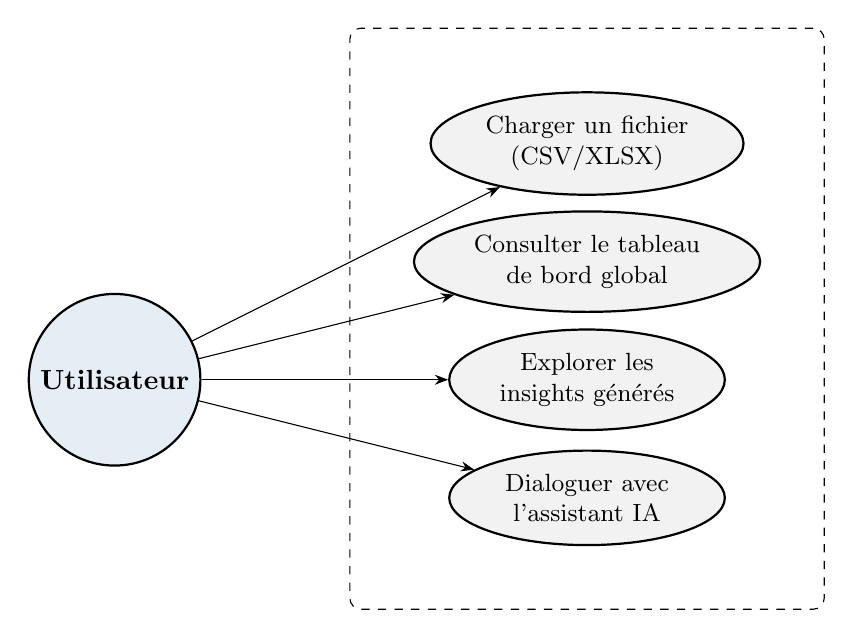
\begin{tikzpicture}[
    actor/.style={draw, circle, minimum size=1cm, fill=bleuUM5!10, thick},
    usecase/.style={draw, ellipse, minimum width=3.5cm, minimum height=1.2cm, fill=bg, thick, align=center, font=\small},
    system/.style={draw, dashed, rounded corners=10pt, inner sep=15pt, fill=bleuUM5!3}
]
\node[actor] (user) at (0,0) {\textbf{Utilisateur}};

\node[usecase] (uc1) at (6,3) {Charger un fichier\\(CSV/XLSX)};
\node[usecase] (uc2) at (6,1.5) {Consulter le tableau\\de bord global};
\node[usecase] (uc3) at (6,0) {Explorer les\\insights générés};
\node[usecase] (uc4) at (6,-1.5) {Dialoguer avec\\l'assistant IA};
% \node[usecase] (uc5) at (6,-3) {Filtrer par période};

% Cadre système (dessiné après mais en arrière-plan)
\begin{pgfonlayer}{background}
\node[
    draw,
    dashed,
    rounded corners,
    fit=(uc1)(uc2)(uc3)(uc4),
    inner sep=0.8cm
] {};
\end{pgfonlayer}

\draw[-{Stealth}] (user) -- (uc1);
\draw[-{Stealth}] (user) -- (uc2);
\draw[-{Stealth}] (user) -- (uc3);
\draw[-{Stealth}] (user) -- (uc4);
% \draw[-{Stealth}] (user) -- (uc5);
\end{tikzpicture}
\caption{Diagramme de cas d'utilisation du système SmartBI}
\label{fig:usecase}
\end{figure}

\section{Exigences non fonctionnelles}

\subsection{Performance}

Le temps d'ingestion d'un fichier de 10~000 lignes ne doit pas excéder 5 secondes. Le temps de génération d'un tableau de bord par le pipeline d'agents doit rester inférieur à 60 secondes pour un jeu de données de taille modérée. L'interface utilisateur doit offrir un temps de chargement initial inférieur à 3 secondes sur une connexion locale.

\subsection{Sécurité et confidentialité}

Les données utilisateur sont traitées exclusivement en local, sans transfert vers des services cloud. Les fichiers uploadés sont limités à 10~Mo. Les noms de colonnes sont normalisés pour prévenir les injections SQL. Les modèles de langage sont exécutés localement via Ollama, garantissant qu'aucune donnée sensible ne quitte l'infrastructure de l'utilisateur.

\subsection{Maintenabilité}

L'architecture sépare clairement le frontend et le backend via une API REST, facilitant l'évolution indépendante de chaque couche. Les prompts des agents IA sont externalisés dans des templates modifiables sans altérer la logique du pipeline.

\section{Architecture globale du système}

\subsection{Vue d'ensemble}

Le système SmartBI adopte une architecture client-serveur à deux tiers, illustrée par la figure~\ref{fig:archi-globale}. Le frontend React communique avec le backend Django via une API REST. Le backend orchestre le pipeline d'agents LangGraph et interagit avec la base de données SQLite ainsi qu'avec le serveur Ollama pour l'inférence des modèles de langage.

\begin{figure}[H]
\centering
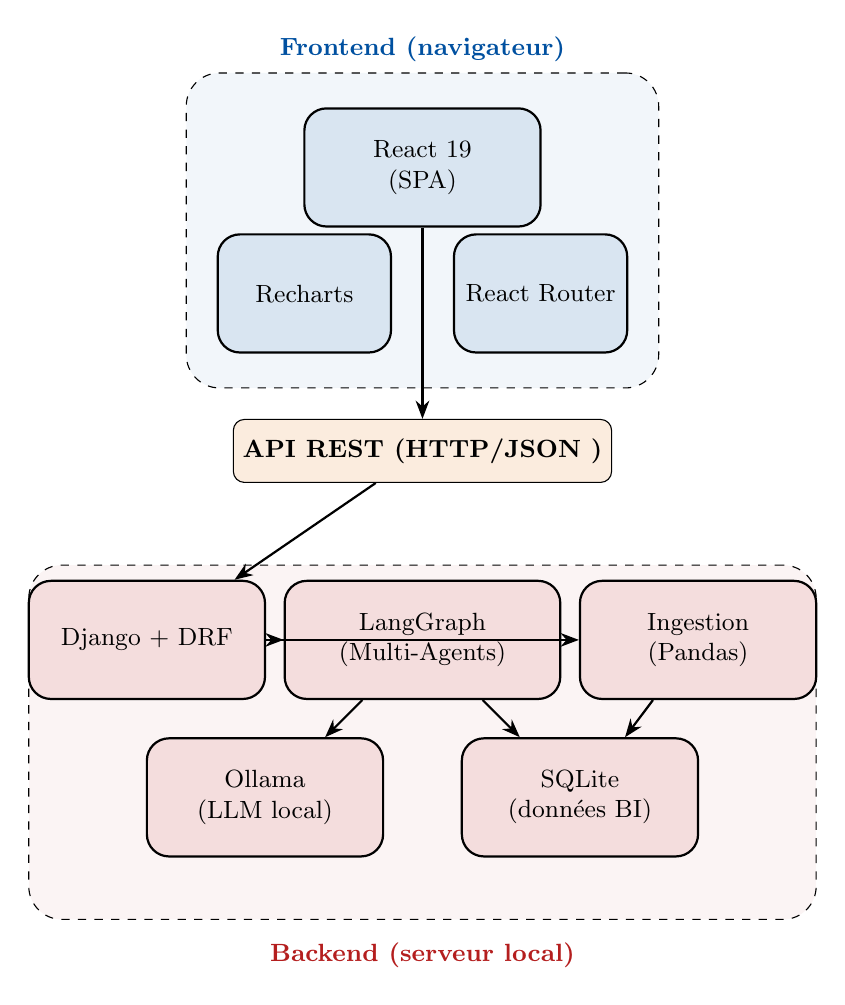
\begin{tikzpicture}[
    box/.style={draw, rounded corners=8pt, minimum width=3cm, minimum height=1.5cm, align=center, font=\small, thick},
    layer/.style={draw, dashed, rounded corners=12pt, inner sep=12pt}
]
% Frontend
\node[layer, fill=bleuUM5!5, minimum width=6cm, minimum height=4cm] (fl) at (0,4) {};
\node[box, fill=bleuUM5!15] (react) at (0,4.8) {React 19\\(SPA)};
\node[box, fill=bleuUM5!15, minimum width=2.2cm] (recharts) at (-1.5,3.2) {Recharts};
\node[box, fill=bleuUM5!15, minimum width=2.2cm] (router) at (1.5,3.2) {React Router};

% Communication
\node[draw, fill=orangecode!15, rounded corners, minimum width=4cm, minimum height=0.8cm, font=\small\bfseries] (api) at (0,1.2) {API REST (HTTP/JSON )};
% + NDJSON
% Backend
\node[layer, fill=rougeENSIAS!5, minimum width=10cm, minimum height=4.5cm] (bl) at (0,-2.5) {};
\node[box, fill=rougeENSIAS!15] (django) at (-3.5,-1.2) {Django + DRF};
\node[box, fill=rougeENSIAS!15, minimum width=3.5cm] (langgraph) at (0,-1.2) {LangGraph\\(Multi-Agents)};
\node[box, fill=rougeENSIAS!15] (ingestion) at (3.5,-1.2) {Ingestion\\(Pandas)};
\node[box, fill=rougeENSIAS!15] (ollama) at (-2,-3.2) {Ollama\\(LLM local)};
\node[box, fill=rougeENSIAS!15] (sqlite) at (2,-3.2) {SQLite\\(données BI)};

\draw[-{Stealth}, thick] (react) -- (api);
\draw[-{Stealth}, thick] (api) -- (django);
\draw[-{Stealth}, thick] (django) -- (langgraph);
\draw[-{Stealth}, thick] (django) -- (ingestion);
\draw[-{Stealth}, thick] (langgraph) -- (ollama);
\draw[-{Stealth}, thick] (ingestion) -- (sqlite);
\draw[-{Stealth}, thick] (langgraph) -- (sqlite);

\node[font=\small\bfseries\color{bleuUM5}] at (0,6.3) {Frontend (navigateur)};
\node[font=\small\bfseries\color{rougeENSIAS}] at (0,-5.2) {Backend (serveur local)};
\end{tikzpicture}
\caption{Architecture globale du système SmartBI}
\label{fig:archi-globale}
\end{figure}

\subsection{Justification des choix architecturaux}

Le choix d'une architecture à deux tiers s'explique par la nature du projet : un prototype fonctionnel destiné à démontrer la faisabilité de l'approche. La simplicité de déploiement (un serveur Django et un serveur de développement Vite) constitue un avantage significatif. La séparation frontend/backend via une API REST permet néanmoins une évolution future vers une architecture plus distribuée.
%  Le protocole de streaming NDJSON pour l'upload offre une expérience réactive sans nécessiter de WebSocket.

\section{Conception du pipeline multi-agents}

\subsection{Vue d'ensemble du pipeline LangGraph}

Le cœur du système repose sur un graphe d'état LangGraph composé de trois nœuds principaux et d'un mécanisme de branchement conditionnel. Ce pipeline est invoqué dans deux contextes : lors du chargement d'un fichier (mode automatique) et lors d'une interaction conversationnelle (mode conversationnel). La figure~\ref{fig:pipeline} illustre le flux d'exécution.

\begin{figure}[H]
\centering
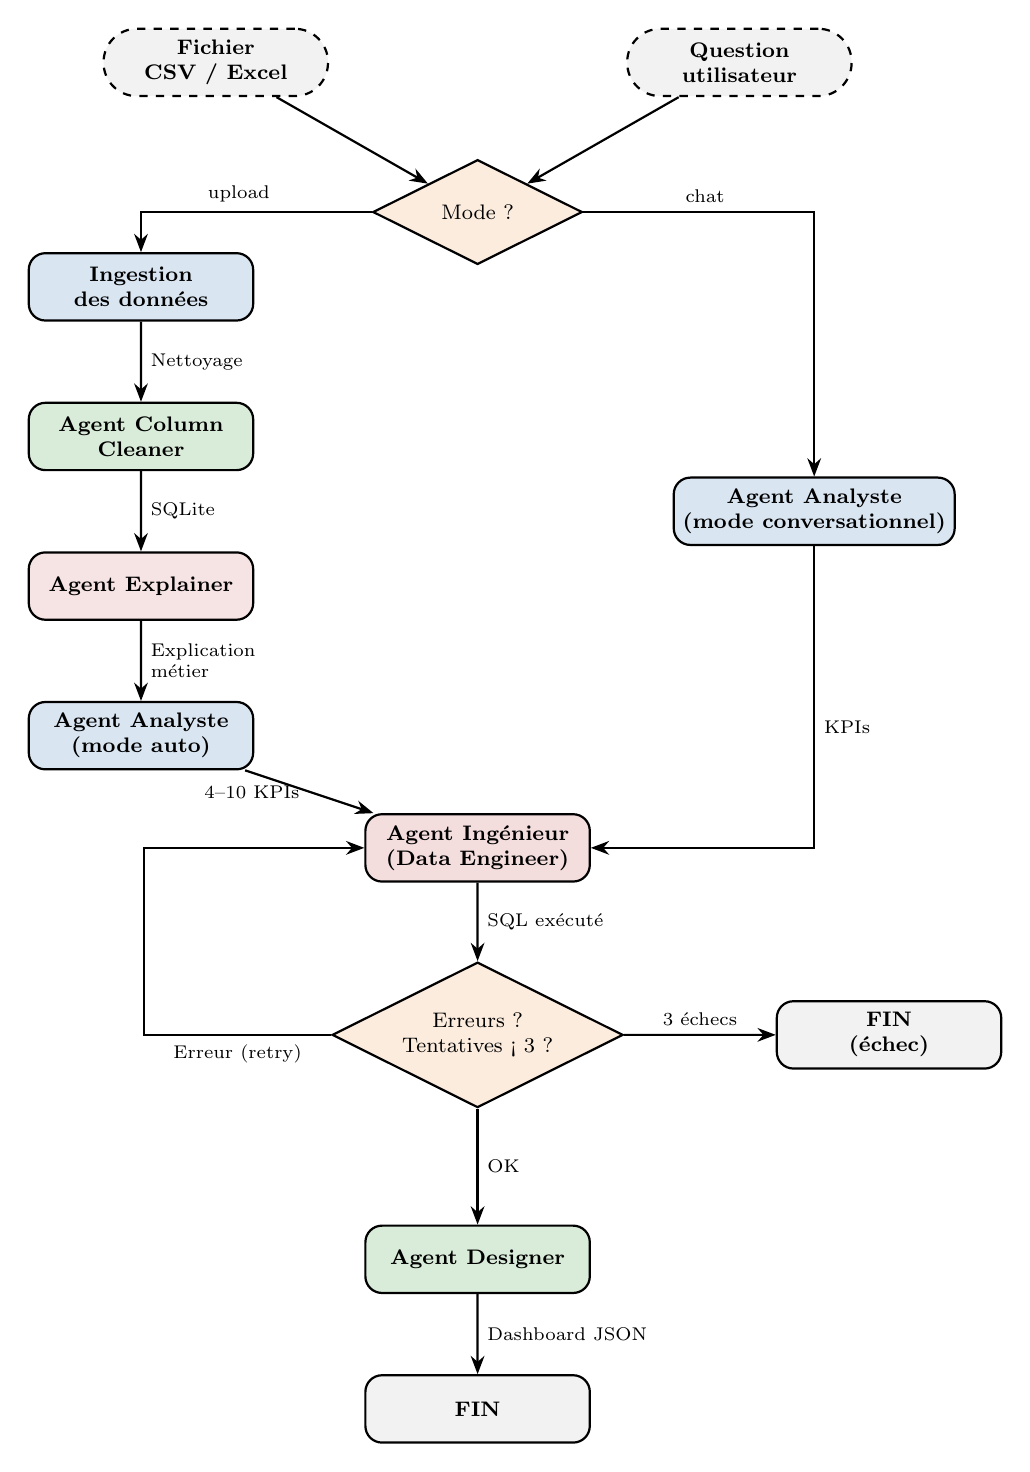
\begin{tikzpicture}[
    scale=0.95,
    transform shape,
    node/.style={
        draw,
        rounded corners=6pt,
        minimum width=3cm,
        minimum height=0.9cm,
        align=center,
        font=\footnotesize\bfseries,
        thick
    },
    edge/.style={-{Stealth}, thick},
    decision/.style={
        draw,
        diamond,
        aspect=2,
        minimum width=2.8cm,
        minimum height=1.4cm,
        align=center,
        font=\footnotesize,
        thick
    },
    entry/.style={
        draw,
        rounded corners=12pt,
        minimum width=3cm,
        minimum height=0.9cm,
        align=center,
        font=\footnotesize\bfseries,
        thick,
        dashed
    }
]

% === Entrées utilisateur ===
\node[entry, fill=gray!10] (upload) at (-3.5, 0)
{Fichier\\CSV / Excel};

\node[entry, fill=gray!10] (question) at (3.5, 0)
{Question\\utilisateur};

% === Mode décision ===
\node[decision, fill=orangecode!15] (mode) at (0, -2)
{Mode ?};

% === Branche Upload (gauche) ===
\node[node, fill=bleuUM5!15] (ingestion) at (-4.5, -3)
{Ingestion\\des données};

\node[node, fill=vertcode!15] (cleaner) at (-4.5, -5)
{Agent Column\\Cleaner};

\node[node, fill=rougeENSIAS!12] (explainer) at (-4.5, -7)
{Agent Explainer};

\node[node, fill=bleuUM5!15] (autoanalyst) at (-4.5, -9)
{Agent Analyste\\(mode auto)};

% === Branche Chat (droite) ===
\node[node, fill=bleuUM5!15] (convanalyst) at (4.5, -6)
{Agent Analyste\\(mode conversationnel)};

% === Tronc commun ===
\node[node, fill=rougeENSIAS!15] (engineer) at (0, -10.5)
{Agent Ingénieur\\(Data Engineer)};

\node[decision, fill=orangecode!15] (check) at (0, -13)
{Erreurs ?\\Tentatives < 3 ?};

\node[node, fill=vertcode!15] (designer) at (0, -16)
{Agent Designer};

\node[node, fill=bg] (end) at (0, -18)
{FIN};

\node[node, fill=bg] (endfail) at (5.5, -13)
{FIN\\(échec)};

% === Flux : Entrées vers décision ===
\draw[edge] (upload) -- (mode);
\draw[edge] (question) -- (mode);

% === Branche Upload ===
\draw[edge] (mode.west) -| node[above left, font=\scriptsize, pos=0.2] {upload} (ingestion);
\draw[edge] (ingestion) -- node[right, font=\scriptsize] {Nettoyage} (cleaner);
\draw[edge] (cleaner) -- node[right, font=\scriptsize] {SQLite} (explainer);
\draw[edge] (explainer) -- node[right, font=\scriptsize, align=left] {Explication\\métier} (autoanalyst);
\draw[edge] (autoanalyst) -- node[left, font=\scriptsize] {4--10 KPIs} (engineer);

% === Branche Chat ===
\draw[edge] (mode.east) -| node[above right, font=\scriptsize, pos=0.2] {chat} (convanalyst);
\draw[edge] (convanalyst) |- node[right, font=\scriptsize, pos=0.3] {KPIs} (engineer);

% === Tronc commun ===
\draw[edge] (engineer) -- node[right, font=\scriptsize] {SQL exécuté} (check);

% OK vers Designer
\draw[edge] (check.south) -- node[right, font=\scriptsize] {OK} (designer);

% Retry
\draw[edge] (check.west) -- ++(-2.5,0) node[below, font=\scriptsize, pos=0.5] {Erreur (retry)} |- (engineer.west);

% Échec définitif
\draw[edge] (check.east) -- node[above, font=\scriptsize] {3 échecs} (endfail);

% Designer vers FIN
\draw[edge] (designer) -- node[right, font=\scriptsize] {Dashboard JSON} (end);

\end{tikzpicture}
\caption{Pipeline complet du système SmartBI : ingestion, agents IA et mécanisme de retry}
\label{fig:pipeline-complet}
\end{figure}


\subsection{État partagé du graphe}

Le graphe LangGraph est paramétré par un état partagé qui évolue au fur et à mesure que les agents produisent leurs résultats. Le tableau~\ref{tab:graphstate} détaille les champs de cet état.

\begin{table}[H]
\centering
\renewcommand{\arraystretch}{1.5} % Aère le tableau pour éviter que le texte ne touche les lignes
\caption{Structure de l'état partagé du graphe LangGraph}
\label{tab:graphstate}
\begin{tabularx}{\textwidth}{
    >{\raggedright\arraybackslash\bfseries}l 
    >{\centering\arraybackslash}p{2.8cm} 
    >{\raggedright\arraybackslash}X
}
\toprule
\textbf{Champ} & \textbf{Type} & \textbf{Description} \\
\midrule
mode                 & Literal      & Mode~: \texttt{conversational} ou \texttt{auto} \\
question\_utilisateur & Texte        & Question en langage naturel \\
schema\_db            & Texte        & DDL complet des tables de la base BI \\
kpis\_proposes       & Texte        & Liste des KPIs proposés par l'analyste \\
donnees\_brutes      & Dictionnaire & Résultats bruts des requêtes SQL \\
dashboard\_json      & Texte        & JSON final du tableau de bord \\
erreurs              & Texte        & Messages d'erreur des requêtes SQL échouées \\
tentatives           & Entier       & Compteur de tentatives (max 3) \\
\bottomrule
\end{tabularx}
\end{table}

\subsection{Agent Column Cleaner}
Intervenant juste après l'ingestion initiale par Pandas et avant l'écriture dans la base SQLite, l'agent Column Cleaner agit comme un \textit{Data Engineer expert en qualité de données}. Il analyse un échantillon des données ainsi que leurs statistiques descriptives pour identifier et suggérer la suppression des colonnes inutiles (identifiants redondants, colonnes quasi-vides, constantes ou métadonnées techniques). Ses recommandations sont retournées à l'utilisateur sous forme de JSON structuré pour validation avant l'écriture définitive en base, assurant ainsi une base de données propre et optimisée pour l'analyse BI.

\subsection{Agent Explainer}
L'agent explainer intervient en amont du pipeline LangGraph principal, après la validation du nettoyage et le chargement dans SQLite. Il adopte le rôle d'un \textit{Data Scientist expert} et reçoit en entrée le schéma SQL de la base de données (les instructions \texttt{CREATE TABLE} extraites de SQLite). Son objectif est de rédiger une synthèse courte et professionnelle, en un ou deux paragraphes, expliquant le domaine ou le métier dont proviennent très probablement les données, ainsi que les informations clés exploitables et le potentiel d'analyse qu'elles offrent.
Cet agent ne génère ni code ni JSON : il produit uniquement un texte en langage naturel, affiché ensuite dans la page \textit{Vue Exécutive} du frontend sous l'intitulé « Contexte et domaine des données ». Cette étape permet à l'utilisateur de valider que le système a correctement identifié la nature de ses données avant de consulter les KPIs et visualisations générés par les agents suivants.

\subsection{Agent Analyste}

L'agent analyste est le premier nœud du graphe. Il dispose de deux modes de fonctionnement :

\textbf{Mode conversationnel} : l'agent reçoit la question de l'utilisateur et le schéma de la base de données. Il adopte le rôle d'un \textit{Business Analyst Senior} et propose une liste de KPIs réalisables avec les colonnes disponibles, sans générer de SQL.

\textbf{Mode automatique} : activé lors du chargement d'un fichier, il propose 4 à 10 KPIs pour un tableau de bord exécutif, en priorisant les données fraîchement chargées, avec diversité de visualisations et analyses temporelles si des colonnes de type date sont détectées.

\subsection{Agent Ingénieur de données}

L'agent ingénieur traduit les KPIs proposés en requêtes SQLite exécutables. Il génère un dictionnaire associant chaque KPI à une requête SQL valide, en respectant le schéma fourni et la syntaxe SQLite. Les requêtes sont exécutées et les résultats retournés sous forme de dictionnaires.

En cas d'erreurs SQL, celles-ci sont capturées et le mécanisme de retry renvoie l'exécution vers l'agent ingénieur avec les messages d'erreur en contexte, permettant l'auto-correction. Ce cycle est limité à trois tentatives.

\subsection{Agent Designer}

L'agent designer transforme les données brutes en un tableau de bord structuré au format JSON. Il dispose de quatre types de composants visuels : \textbf{MetricCard} (indicateur unique), \textbf{BarChart} (comparaisons catégorielles), \textbf{PieChart} (distributions) et \textbf{LineChart} (évolutions temporelles). Le JSON produit est directement consommable par le frontend.

\subsection{Mécanisme de routage conditionnel}

La logique de contrôle examine l'état après l'agent ingénieur et prend l'une des trois décisions : retour vers l'ingénieur pour retry (si erreurs et tentatives < 3), terminaison du graphe (si 3 échecs), ou passage au designer (si aucune erreur). Ce mécanisme confère au système une résilience notable.

\section{Conception de l'ingestion de données}

Le module d'ingestion prend en charge les fichiers CSV et XLSX et exécute cinq étapes : lecture du fichier par Pandas, normalisation des noms de colonnes, calcul d'un rapport de santé complet (statistiques descriptives), appel à l'Agent Column Cleaner pour suggérer les nettoyages pertinents, puis après validation utilisateur, écriture dans la table \texttt{dataset\_utilisateur} de la base SQLite en mode remplacement.

\section{Conception de l'interface utilisateur}

\subsection{Architecture de navigation}

L'interface est une application monopage (SPA) React avec quatre vues principales : \textbf{Source de données} (\texttt{/upload}) pour le chargement de fichiers, \textbf{Tableau de bord global} (\texttt{/dashboard}) pour la santé des données, \textbf{Insights} (\texttt{/insights}) pour le dashboard généré par les agents avec filtrage temporel, et \textbf{Chat IA} (\texttt{/chat}) pour le dialogue en langage naturel.

\subsection{Gestion de l'état applicatif}

L'état global est géré par un pattern Context + useReducer avec persistance dans le navigateur. Il comprend le rapport de santé des données, le tableau de bord automatique et le tableau de bord conversationnel.

\subsection{Composants de visualisation}

Le moteur de rendu partagé dispose les widgets dans une grille CSS à 12 colonnes responsive. Quatre types de visualisations sont supportés via Recharts : MetricCard, BarChart, PieChart et LineChart, avec formatage français des nombres et calcul de tendances.

\subsection{Interface de chat double mode}

L'assistant IA est accessible via un panneau latéral (420 px, bouton flottant) pour une interaction sans quitter la page courante, et une page dédiée plein écran pour une conversation immersive. Les deux modes partagent le même état.

\section{Conception de la base de données}

Le système utilise deux bases SQLite distinctes : une pour les métadonnées Django (non utilisée activement) et une pour les données métier, dont le chemin est configurable. Le schéma est découvert dynamiquement à l'exécution, permettant au pipeline d'agents de s'adapter à n'importe quelle structure de données. La table \texttt{dataset\_utilisateur} est remplacée à chaque nouvel upload.

\section{Synthèse}

La conception repose sur trois piliers : un pipeline multi-agents LangGraph avec séparation des responsabilités, une interface réactive et intuitive, et une architecture de stockage flexible avec découverte dynamique de schéma. Le chapitre suivant détaille la mise en œuvre technique.

%==============================================================================
% CHAPITRE 3 : RÉALISATION
%==============================================================================
\chapter{Réalisation}

\section{Environnement de développement}

\subsection{Stack technologique}

Le tableau~\ref{tab:technologies} récapitule l'ensemble des technologies utilisées pour la réalisation du projet.

\begin{table}[H]
\centering
\renewcommand{\arraystretch}{1.4} % Aère les lignes sans surcharger la hauteur du tableau
\caption{Stack technologique du projet SmartBI}
\label{tab:technologies}
\begin{tabularx}{\textwidth}{
    >{\raggedright\arraybackslash\bfseries}l 
    >{\raggedright\arraybackslash}l 
    >{\raggedright\arraybackslash}X
}
\toprule
\textbf{Catégorie} & \textbf{Technologie} & \textbf{Rôle} \\
\midrule
Framework backend  & Django 6.0                 & Framework web Python avec DRF pour l'API REST \\
CORS               & django-cors-headers       & Gestion des requêtes cross-origin \\
Orchestration IA   & LangGraph                  & Framework de graphes d'état pour agents multi-agents \\
LLM local          & Ollama                     & Serveur d'inférence pour modèles de langage locaux \\
Modèle LLM         & Qwen3-Coder                & Modèle de langage utilisé pour l'inférence \\
Prompts            & LangChain (core + ollama)  & Templates de prompts et connecteur LLM \\
Analyse données    & Pandas + openpyxl          & Lecture et transformation de fichiers CSV/XLSX \\
Base de données    & SQLite                     & Stockage léger embarqué pour les données BI \\
Framework frontend & React 19                   & Bibliothèque UI pour l'interface monopage \\
Build tool         & Vite 8                     & Bundler et serveur de développement rapide \\
Routing            & react-router-dom 7         & Routage SPA côté client \\
Visualisation      & Recharts 3.8               & Graphiques interactifs basés sur D3.js \\
IDE                & VS Code                    & Éditeur de code principal \\
Versioning         & Git                        & Suivi des modifications du code source \\
\bottomrule
\end{tabularx}
\end{table}

\subsection{Organisation du projet}

Le projet est organisé en deux modules principaux : le module frontend (\texttt{frontend\_bi/}) contenant l'application React avec ses pages, composants et contexte global, et le module backend (\texttt{pfa\_backend/}) contenant le projet Django avec l'application \texttt{api\_bi} qui héberge le pipeline d'agents, le module d'ingestion et les vues API. Les deux modules communiquent exclusivement via l'API REST.

\section{Réalisation du backend}

\subsection{Configuration et points d'API}

Le backend Django est configuré avec le middleware CORS en tête de chaîne pour autoriser les requêtes depuis le frontend React. Deux endpoints REST sont exposés, présentés dans le tableau~\ref{tab:endpoints}.

\begin{table}[H]
\centering
\renewcommand{\arraystretch}{1.5} % Aère le tableau pour une meilleure lisibilité
\caption{Endpoints de l'API REST SmartBI}
\label{tab:endpoints}
\begin{tabularx}{\textwidth}{
    >{\raggedright\arraybackslash\bfseries}l 
    >{\centering\arraybackslash}p{2cm} 
    >{\raggedright\arraybackslash}X
}
\toprule
\textbf{Endpoint} & \textbf{Méthode} & \textbf{Description} \\
\midrule
/api/upload/   & POST & Ingestion de fichier CSV/XLSX et proposition de nettoyage des colonnes (NDJSON) \\
/api/confirm\_upload/ & POST & Validation du nettoyage, écriture en base et exécution du pipeline d'agents (NDJSON) \\
/api/generate/ & POST & Génération d'un dashboard à partir d'une question en langage naturel \\
\bottomrule
\end{tabularx}
\end{table}

\subsection{Upload avec streaming de progression et nettoyage}

L'upload de fichiers exploite le mécanisme de \texttt{StreamingHttpResponse} de Django pour envoyer des mises à jour de progression en temps réel au format NDJSON (Newline Delimited JSON). L'ingestion se déroule en deux phases : d'abord le téléversement (\texttt{/api/upload/}) où l'Agent Column Cleaner propose des colonnes à supprimer, puis après validation par l'utilisateur (\texttt{/api/confirm\_upload/}), l'écriture en base et l'analyse.

Le frontend lit cette réponse flux par flux via l'API \texttt{ReadableStream} du navigateur, affichant une barre de progression animée avec le nom de l'agent en cours d'exécution. Les étapes de progression incluent : ingestion (10\%), nettoyage des colonnes (25\%), attente de validation (30\%), application des suppressions (35\%), explication par l'IA (40\%), analyse par l'agent analyste (55\%), requêtage par l'agent ingénieur (70\%), conception du dashboard par l'agent designer (85\%), et finalisation (100\%).

\subsection{Pipeline multi-agents LangGraph}

Le pipeline est implémenté comme un graphe d'état LangGraph compilé une seule fois au chargement du module et réutilisé pour chaque requête. Il orchestre trois agents spécialisés : l'analyste qui propose les KPIs, l'ingénieur qui génère et exécute les requêtes SQL, et le designer qui produit le JSON du dashboard. Un mécanisme de retry avec feedback d'erreur permet jusqu'à trois tentatives en cas d'échec SQL.

Cinq templates de prompts distincts, tous rédigés en français, guident les agents dans leurs rôles respectifs : analyste conversationnel, analyste automatique, ingénieur SQL, designer de dashboard et explainer de dataset.

\section{Réalisation du frontend}

\subsection{Architecture de l'application}

L'application React est structurée selon une architecture par pages avec un composant racine définissant le layout global et les routes. Le contexte global (\texttt{BiPlatformContext}) encapsule un \texttt{useReducer} avec persistance dans le navigateur, assurant la continuité entre les sessions.

\subsection{Page de chargement de données}

La page d'accueil offre une zone de glisser-déposer interactive pour les fichiers CSV et XLSX. Après soumission, une barre de progression gradient indique l'avancement du pipeline avec le nom de l'agent actif. À la fin du traitement, l'utilisateur est redirigé automatiquement vers le tableau de bord global.

\begin{figure}[H]
\centering
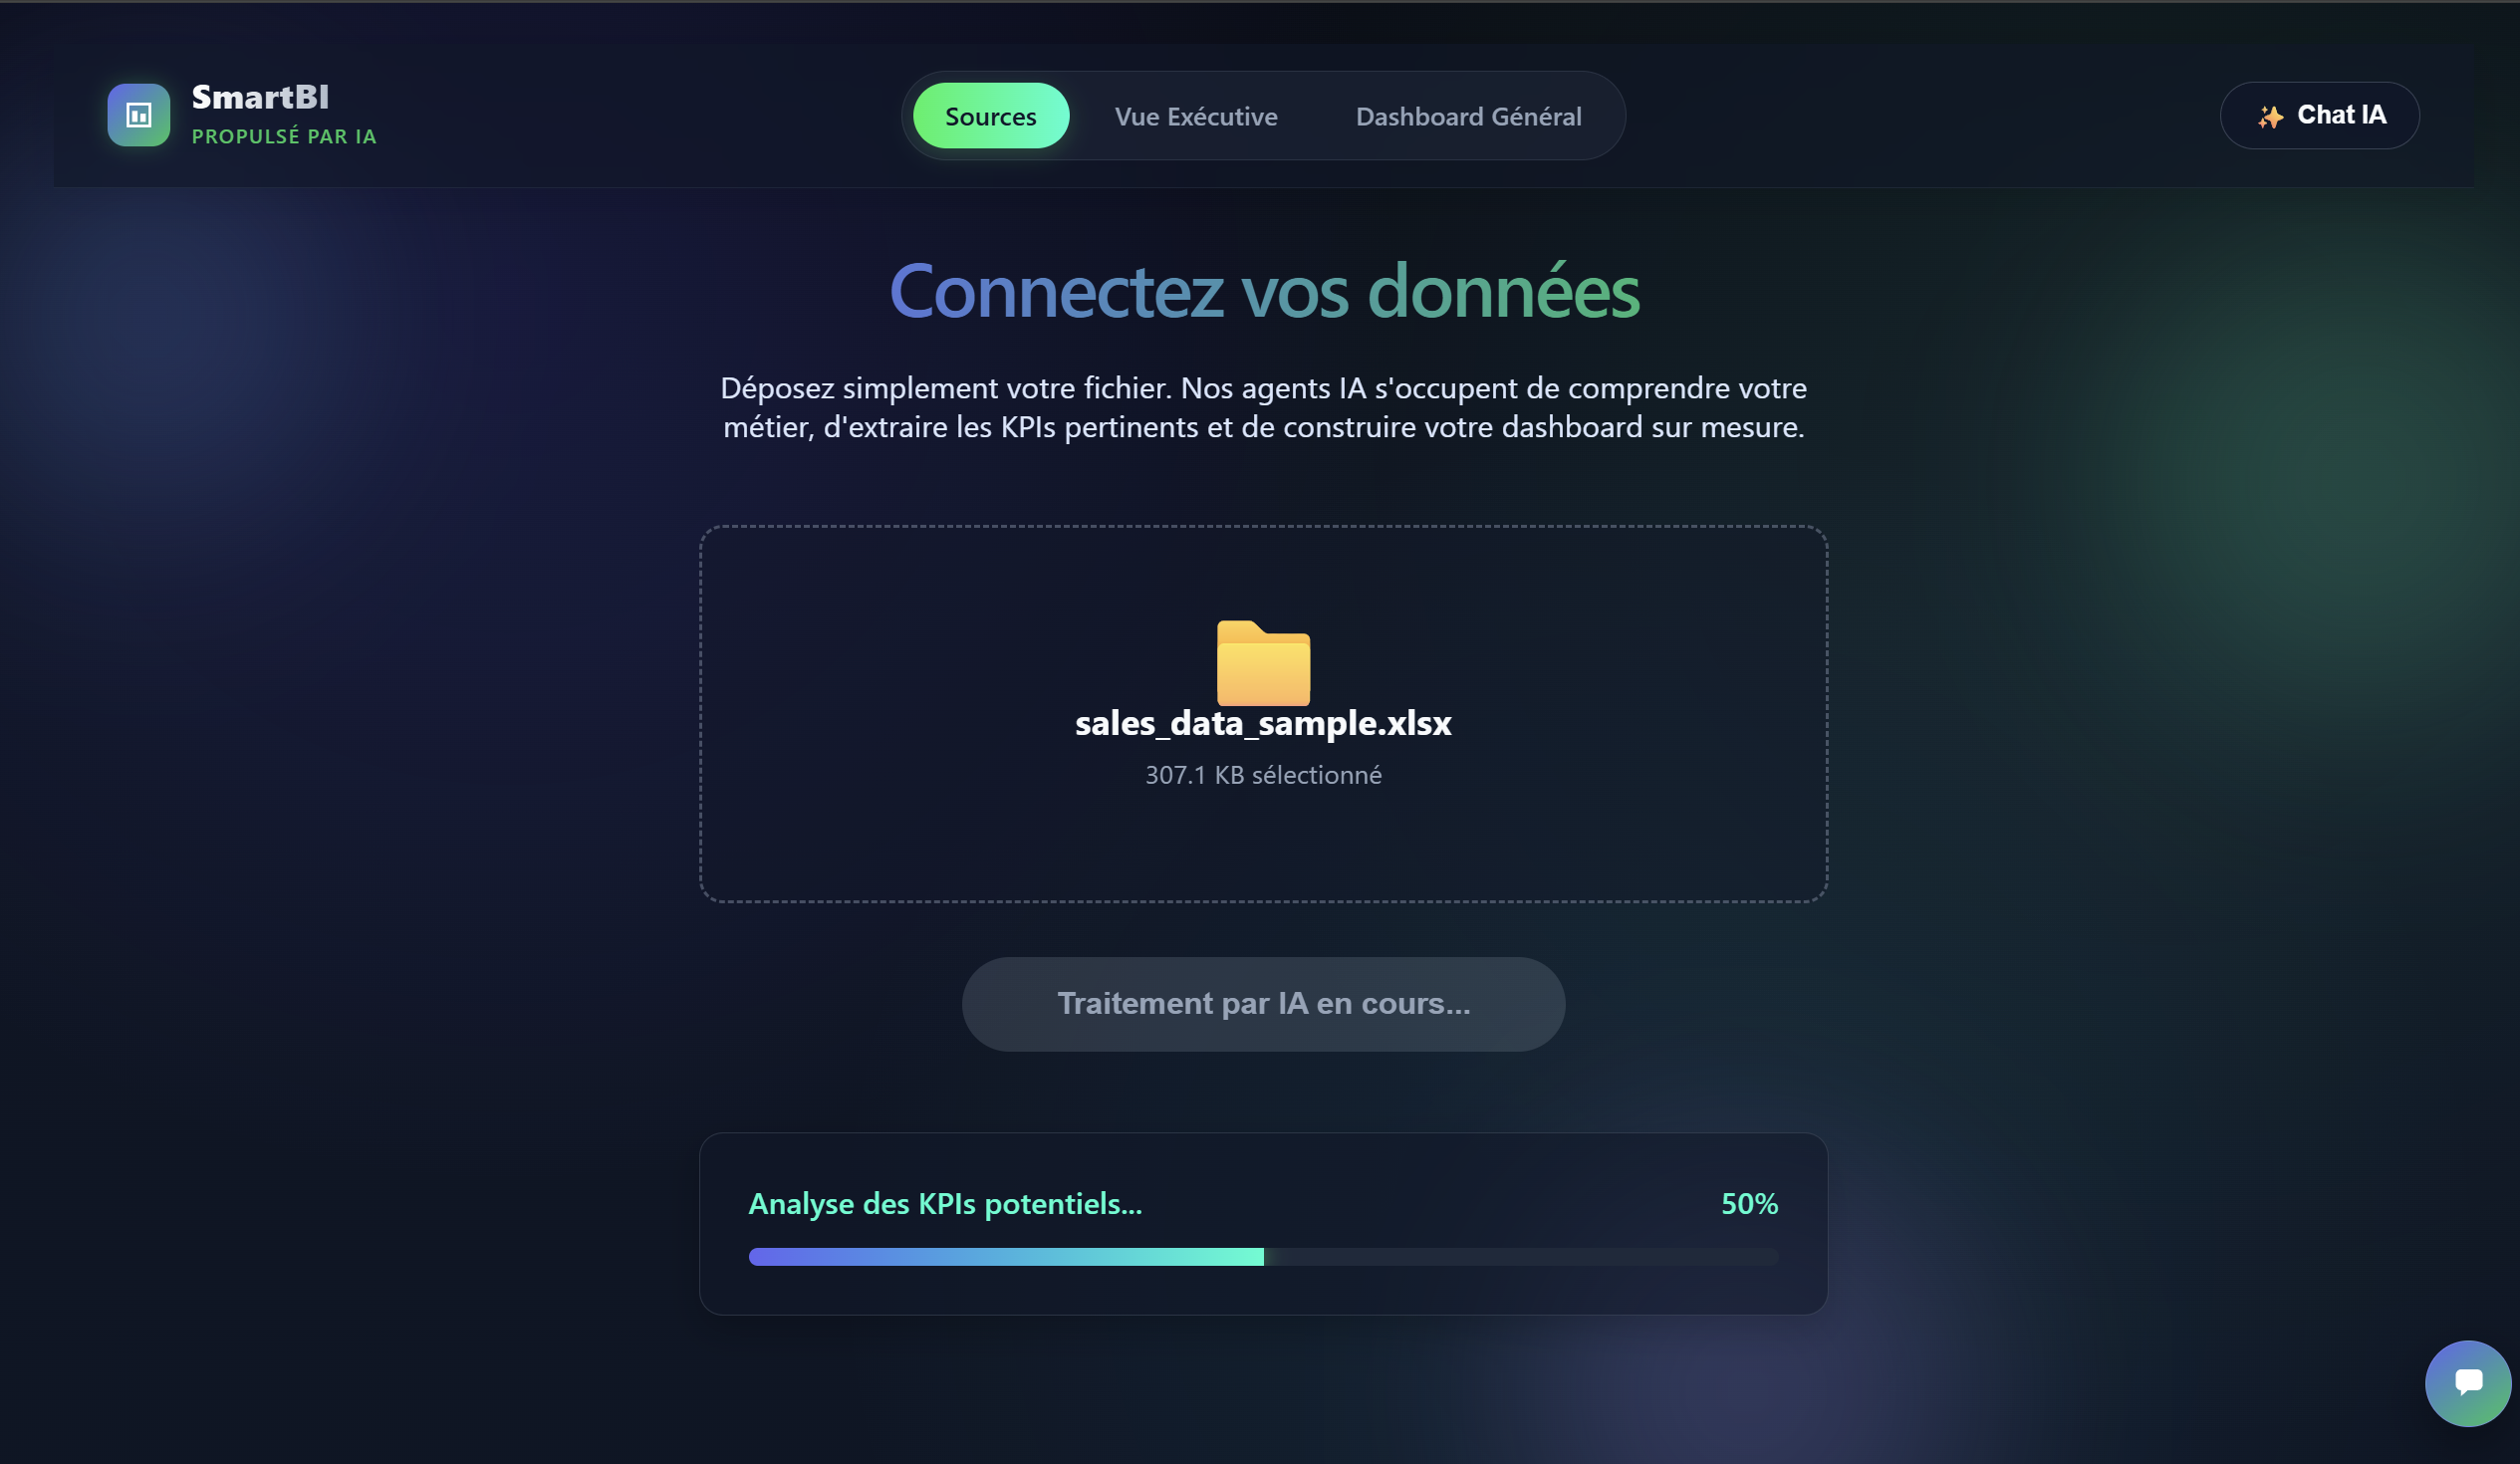
\includegraphics[width=\textwidth]{Smartbi/Screenshot 2026-06-22 173804.png}
\caption{Progression du pipeline d'agents lors de l'upload}
\label{fig:progress}
\end{figure}

\subsection{Tableau de bord global}

Le tableau de bord global présente un résumé exécutif de la santé des données sous forme de six cartes métriques : nombre de lignes, nombre de colonnes, taux de complétude moyen, colonnes numériques, colonnes à risque (nullité $\geq 20\%$) et pourcentage moyen de valeurs nulles. Un panneau d'explication contextuelle générée par l'IA accompagne ces indicateurs, suivi d'un tableau détaillé de chaque colonne avec ses statistiques descriptives.


\begin{figure}[H]
\centering
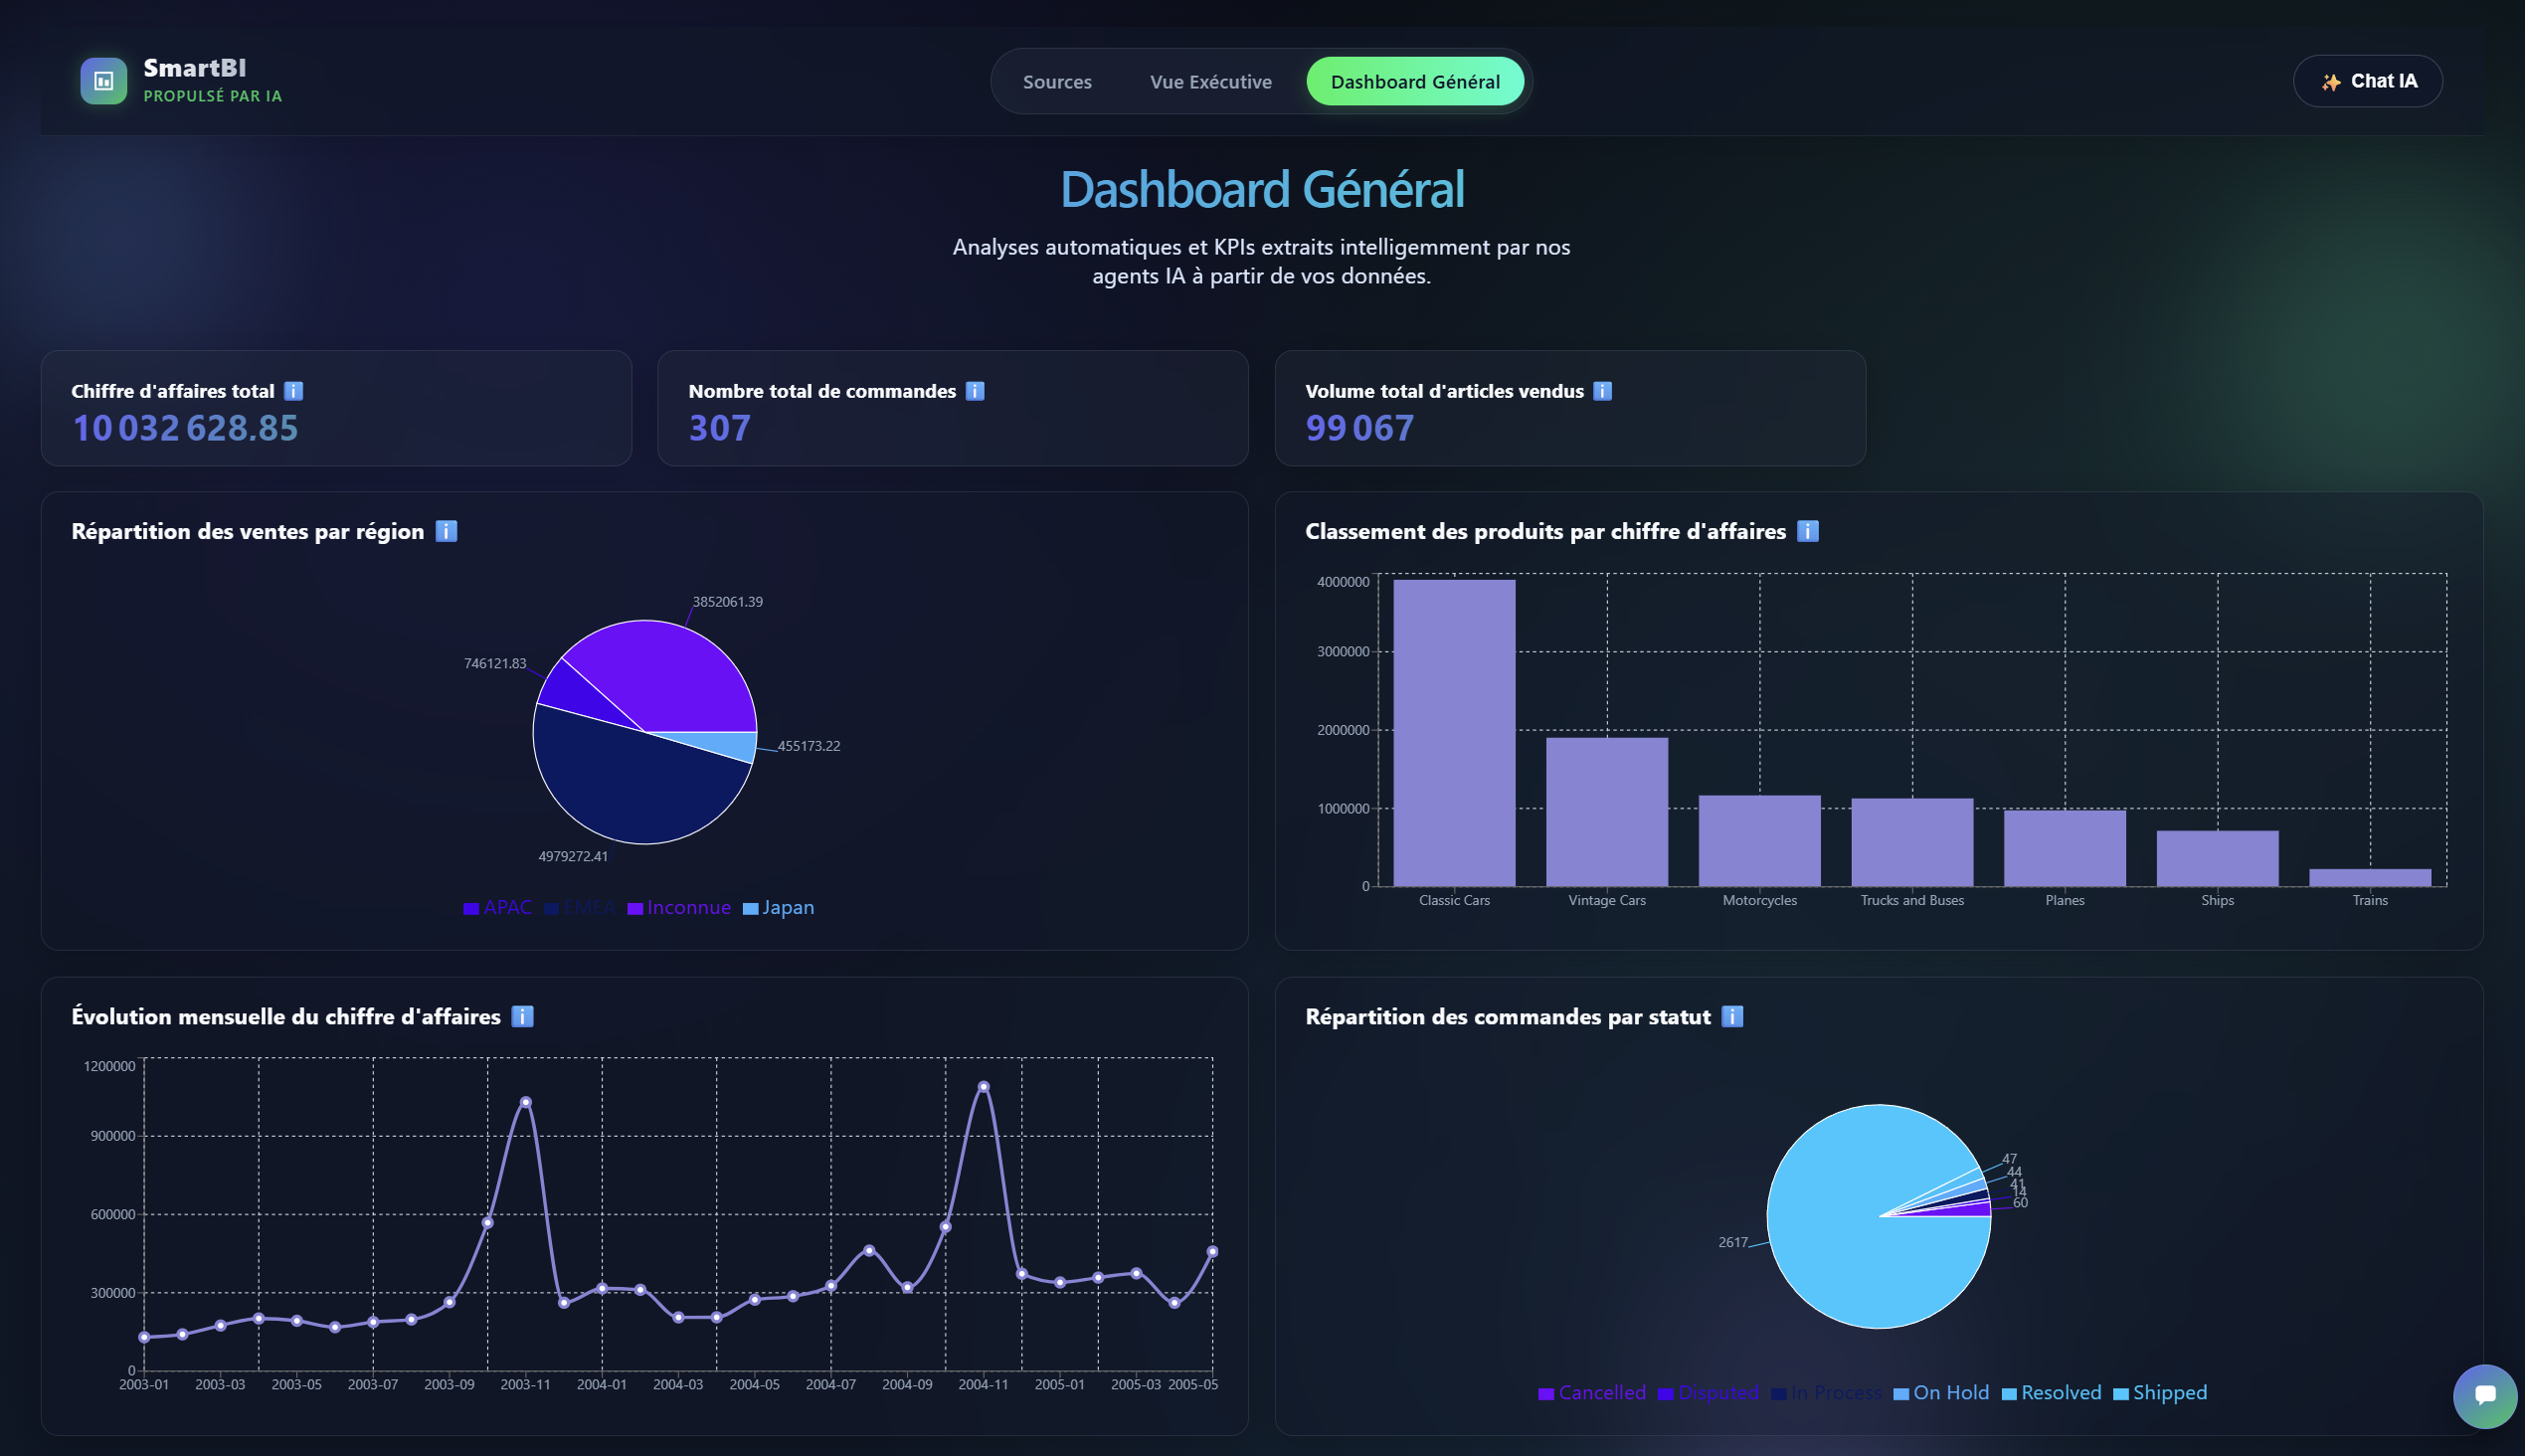
\includegraphics[width=\textwidth]{Smartbi/Screenshot 2026-06-22 181010.png}
\caption{Filtrage temporel dynamique des indicateurs}
\label{fig:filtrage}
\end{figure}

\subsection{Page des insights avec filtrage temporel}

La page des insights rend le tableau de bord généré automatiquement par le pipeline d'agents. Elle implémente un système de filtrage par période qui calcule les options appropriées selon les plages de dates détectées dans les données (jours, mois, années). Les widgets sont disposés dans une grille responsive combinant MetricCards, BarCharts, PieCharts et LineCharts.



\begin{figure}[H]
\centering
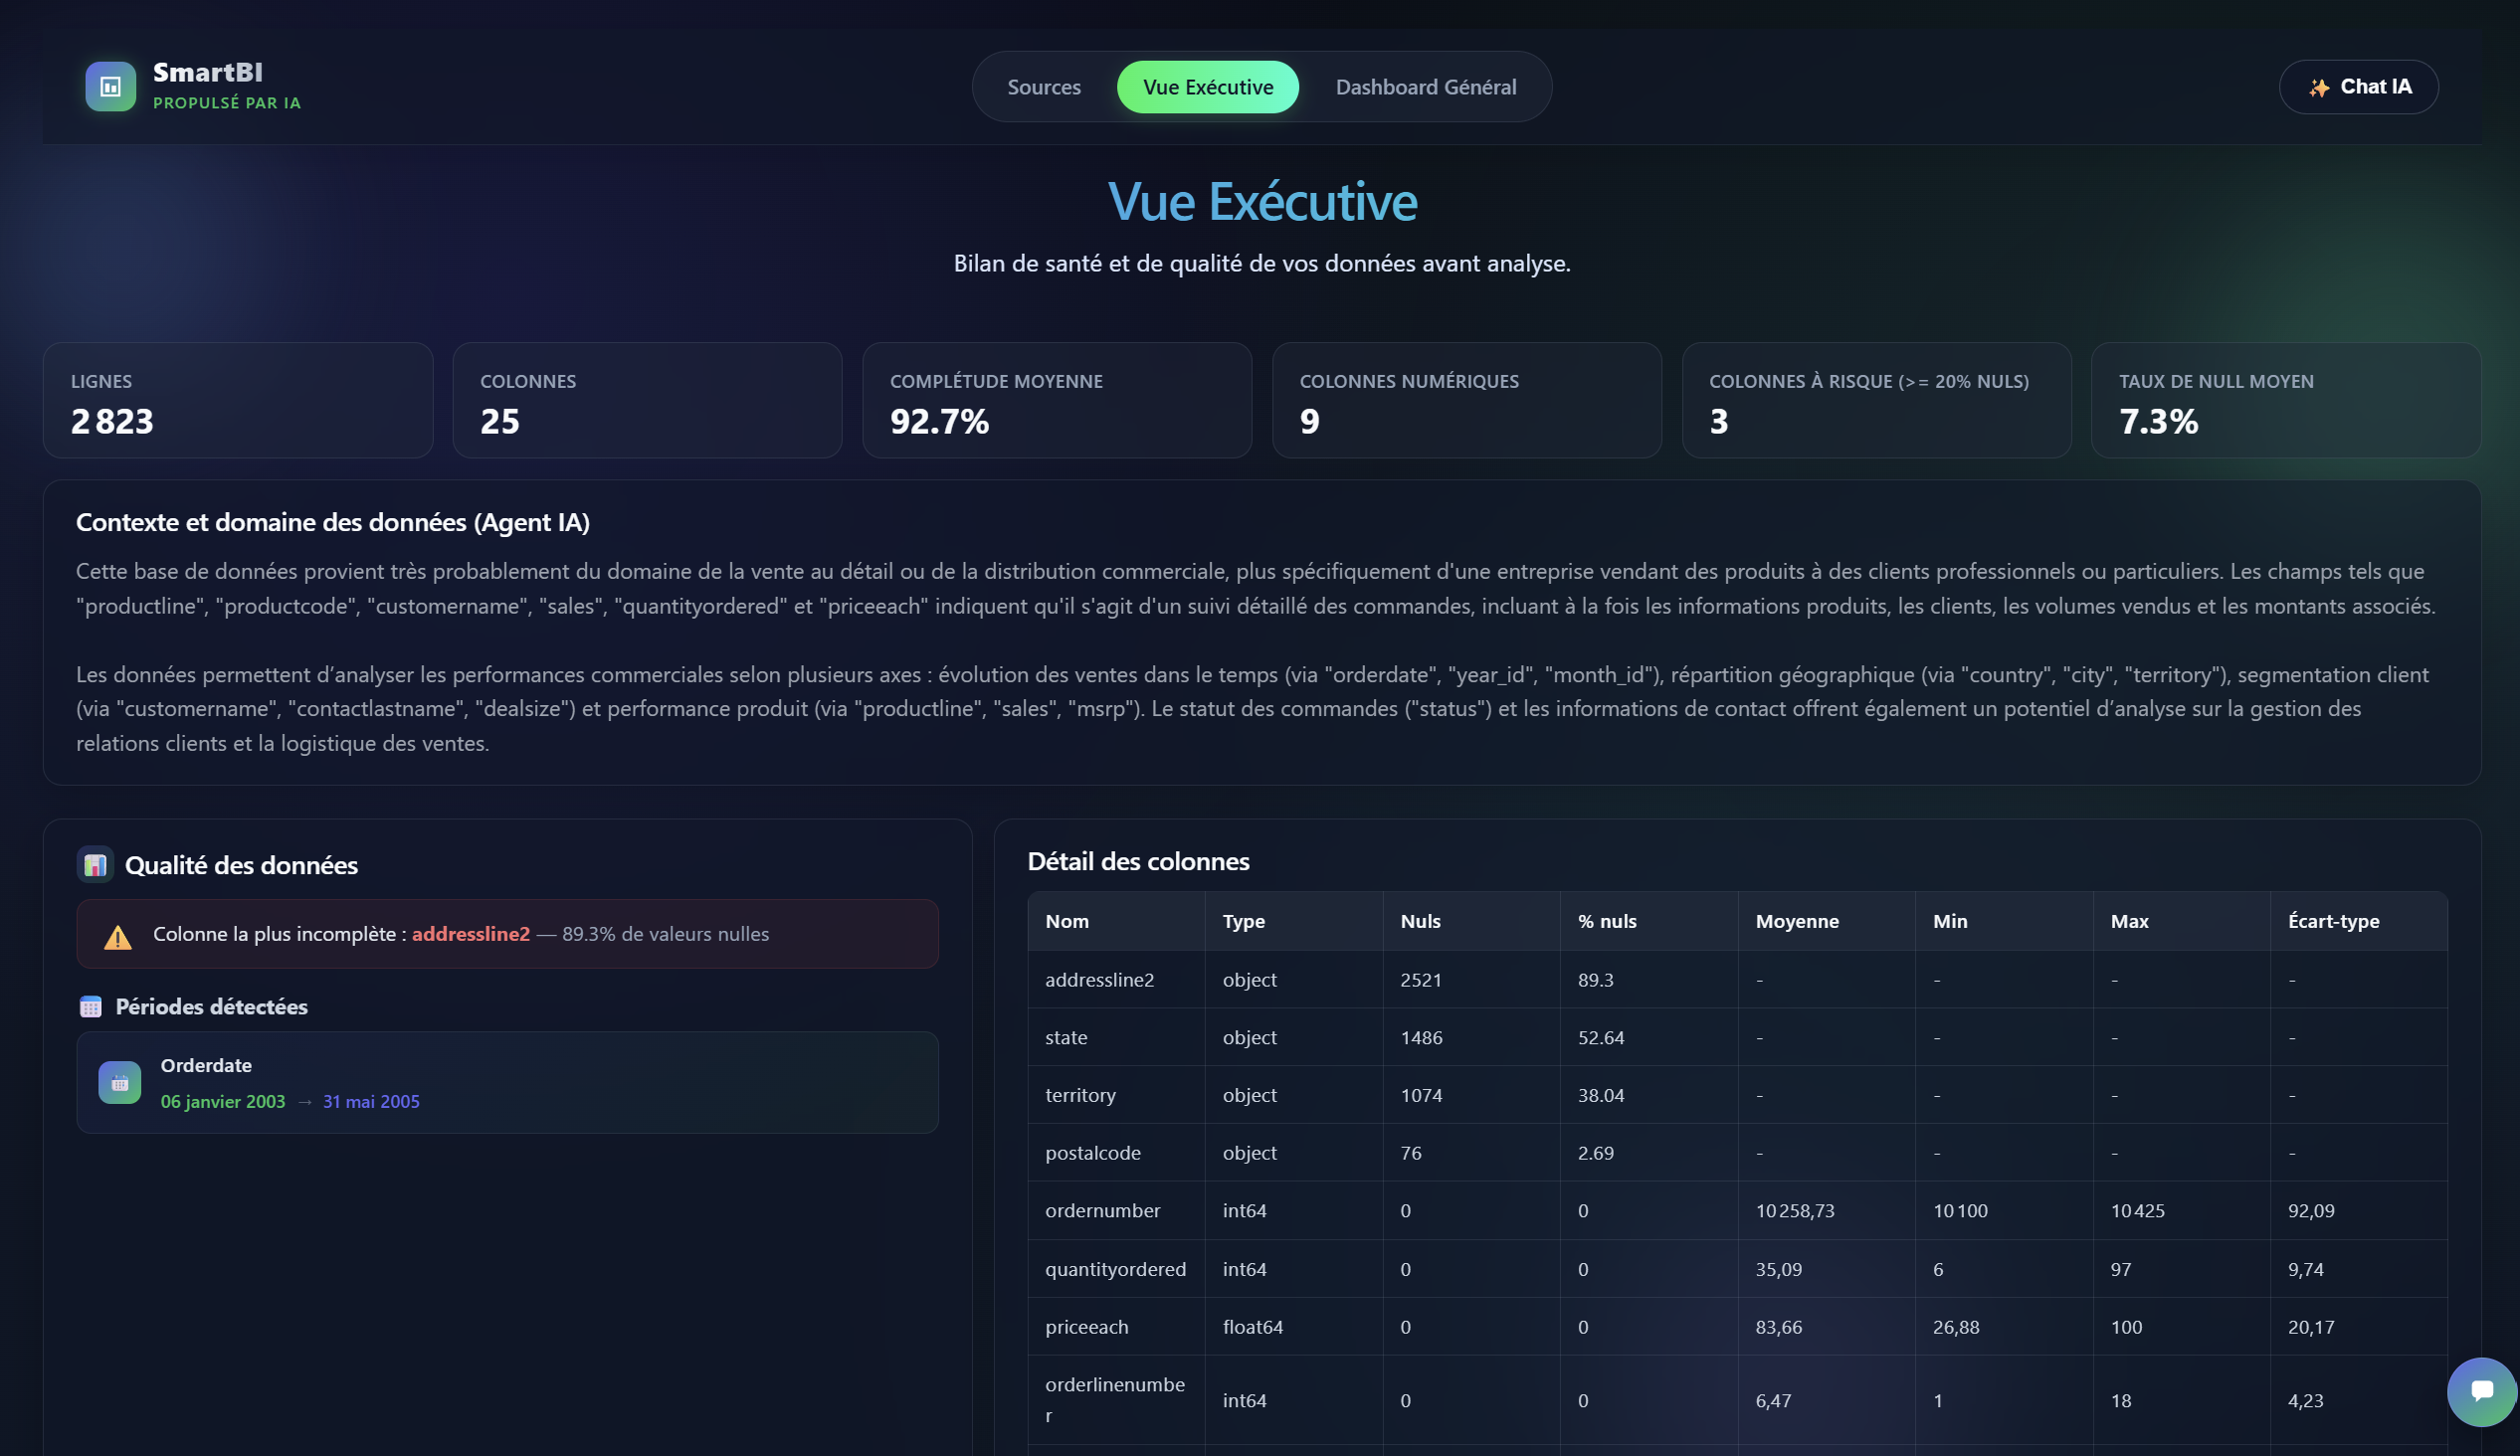
\includegraphics[width=\textwidth]{Smartbi/Screenshot 2026-06-22 180721.png}
\caption{Page des insights --- tableau de bord généré par les agents IA}
\label{fig:filtrage}
\end{figure}

\subsection{Interface de conversation IA}

L'interface de chat offre une expérience conversationnelle fluide avec des bulles de message stylisées et une barre de saisie fixe en bas de page. Afin d'améliorer l'expérience utilisateur et de simuler le temps de réflexion de l'IA, une animation de chargement (trois petits points formant une vague) s'affiche de manière dynamique pendant l'attente de la réponse. Les visualisations générées par l'IA s'affichent ensuite directement dans le fil de conversation, en dessous du message textuel de l'agent. L'assistant est également accessible via un panneau latéral activé par un bouton flottant.



\begin{figure}[H]
\centering
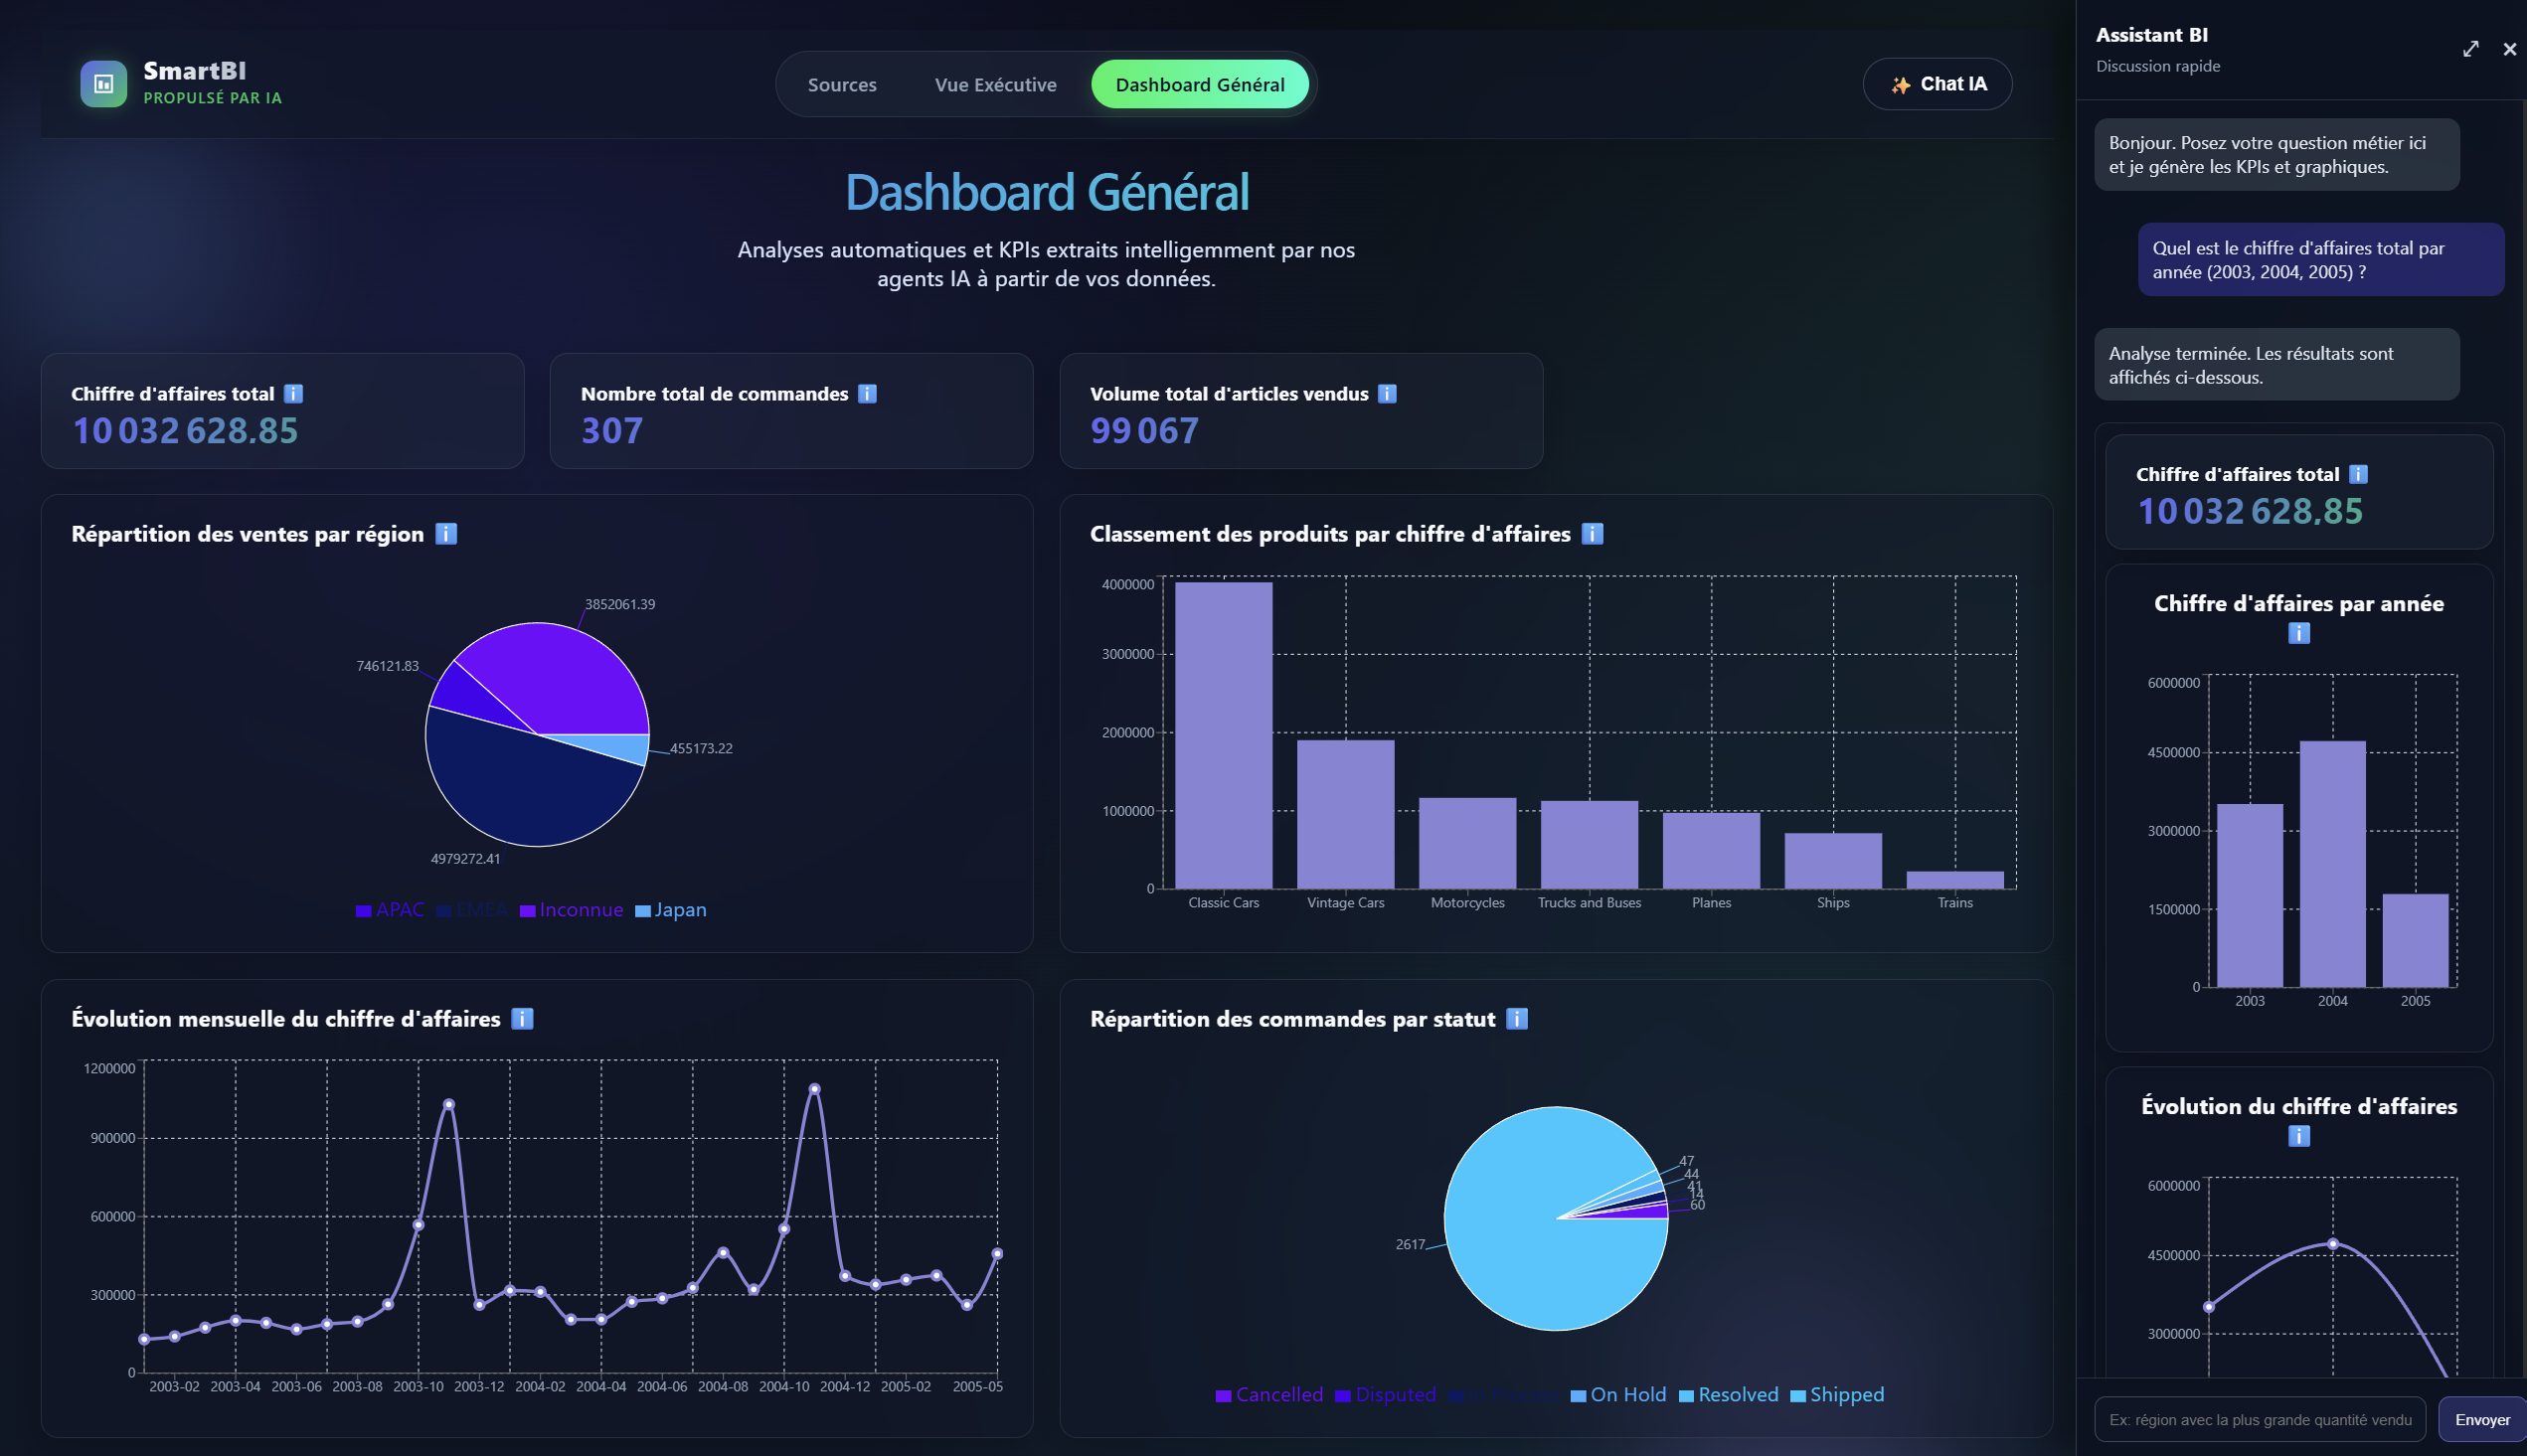
\includegraphics[width=\textwidth]{Smartbi/Screenshot 2026-06-22 181201.png}
\caption{Panneau latéral de conversation IA}
\label{fig:chat-panel}
\end{figure}

\section{Scénarios d'utilisation}

\subsection{Scénario 1 : Analyse automatique d'un fichier de ventes}

Un utilisateur charge un fichier CSV contenant des données de ventes (date, produit, région, quantité, prix unitaire, montant total). Le système ingère les données, génère une explication contextuelle, propose 8 KPIs (chiffre d'affaires total, panier moyen, ventes par région, évolution mensuelle, top 5 produits, etc.), exécute les requêtes SQL et produit un dashboard complet combinant cartes métriques et graphiques variés.


\begin{figure}[H]
\centering
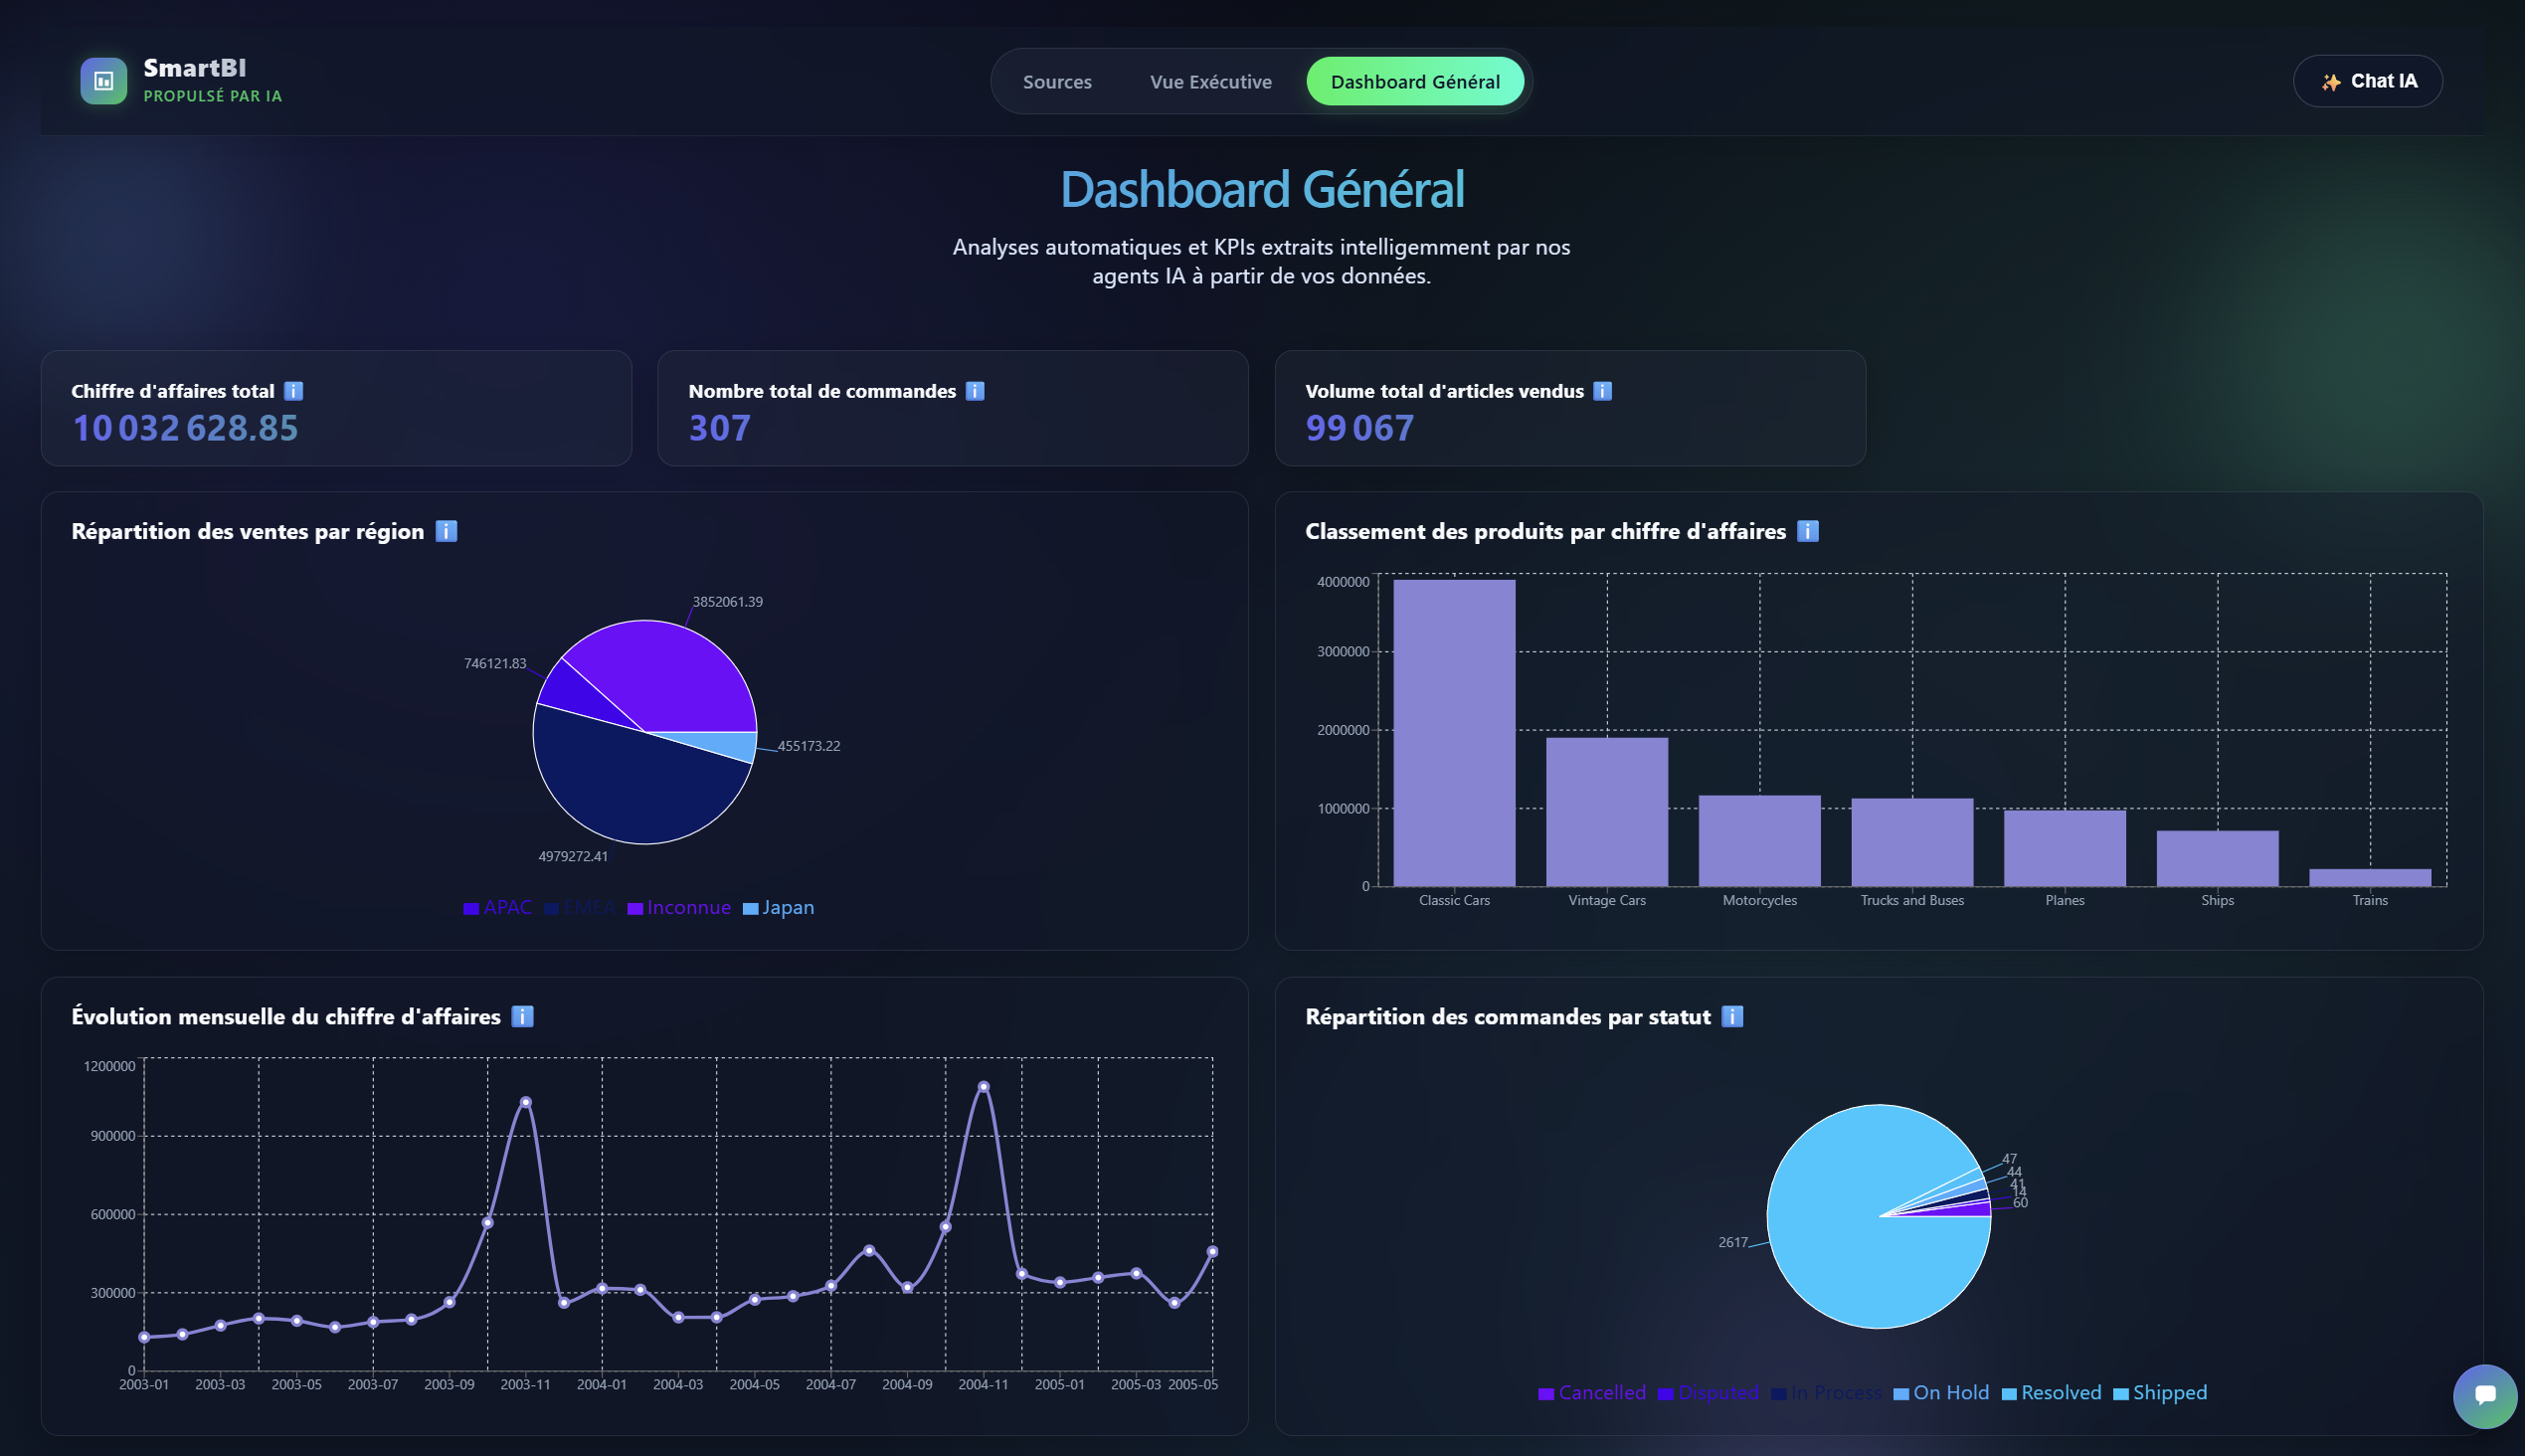
\includegraphics[width=\textwidth]{Smartbi/Screenshot 2026-06-22 181010.png}
\caption{Dashboard généré automatiquement à partir du fichier de ventes}
\label{fig:filtrage}
\end{figure}


\subsection{Scénario 2 : Question conversationnelle}

Après avoir chargé ses données, l'utilisateur pose la question : «~Quel est le produit le plus vendu par mois~?~» Le système active le mode conversationnel, l'analyste identifie le KPI pertinent, l'ingénieur génère la requête SQL avec agrégation mensuelle, et le designer produit un graphique affiché inline dans la conversation.



\begin{figure}[H]
\centering
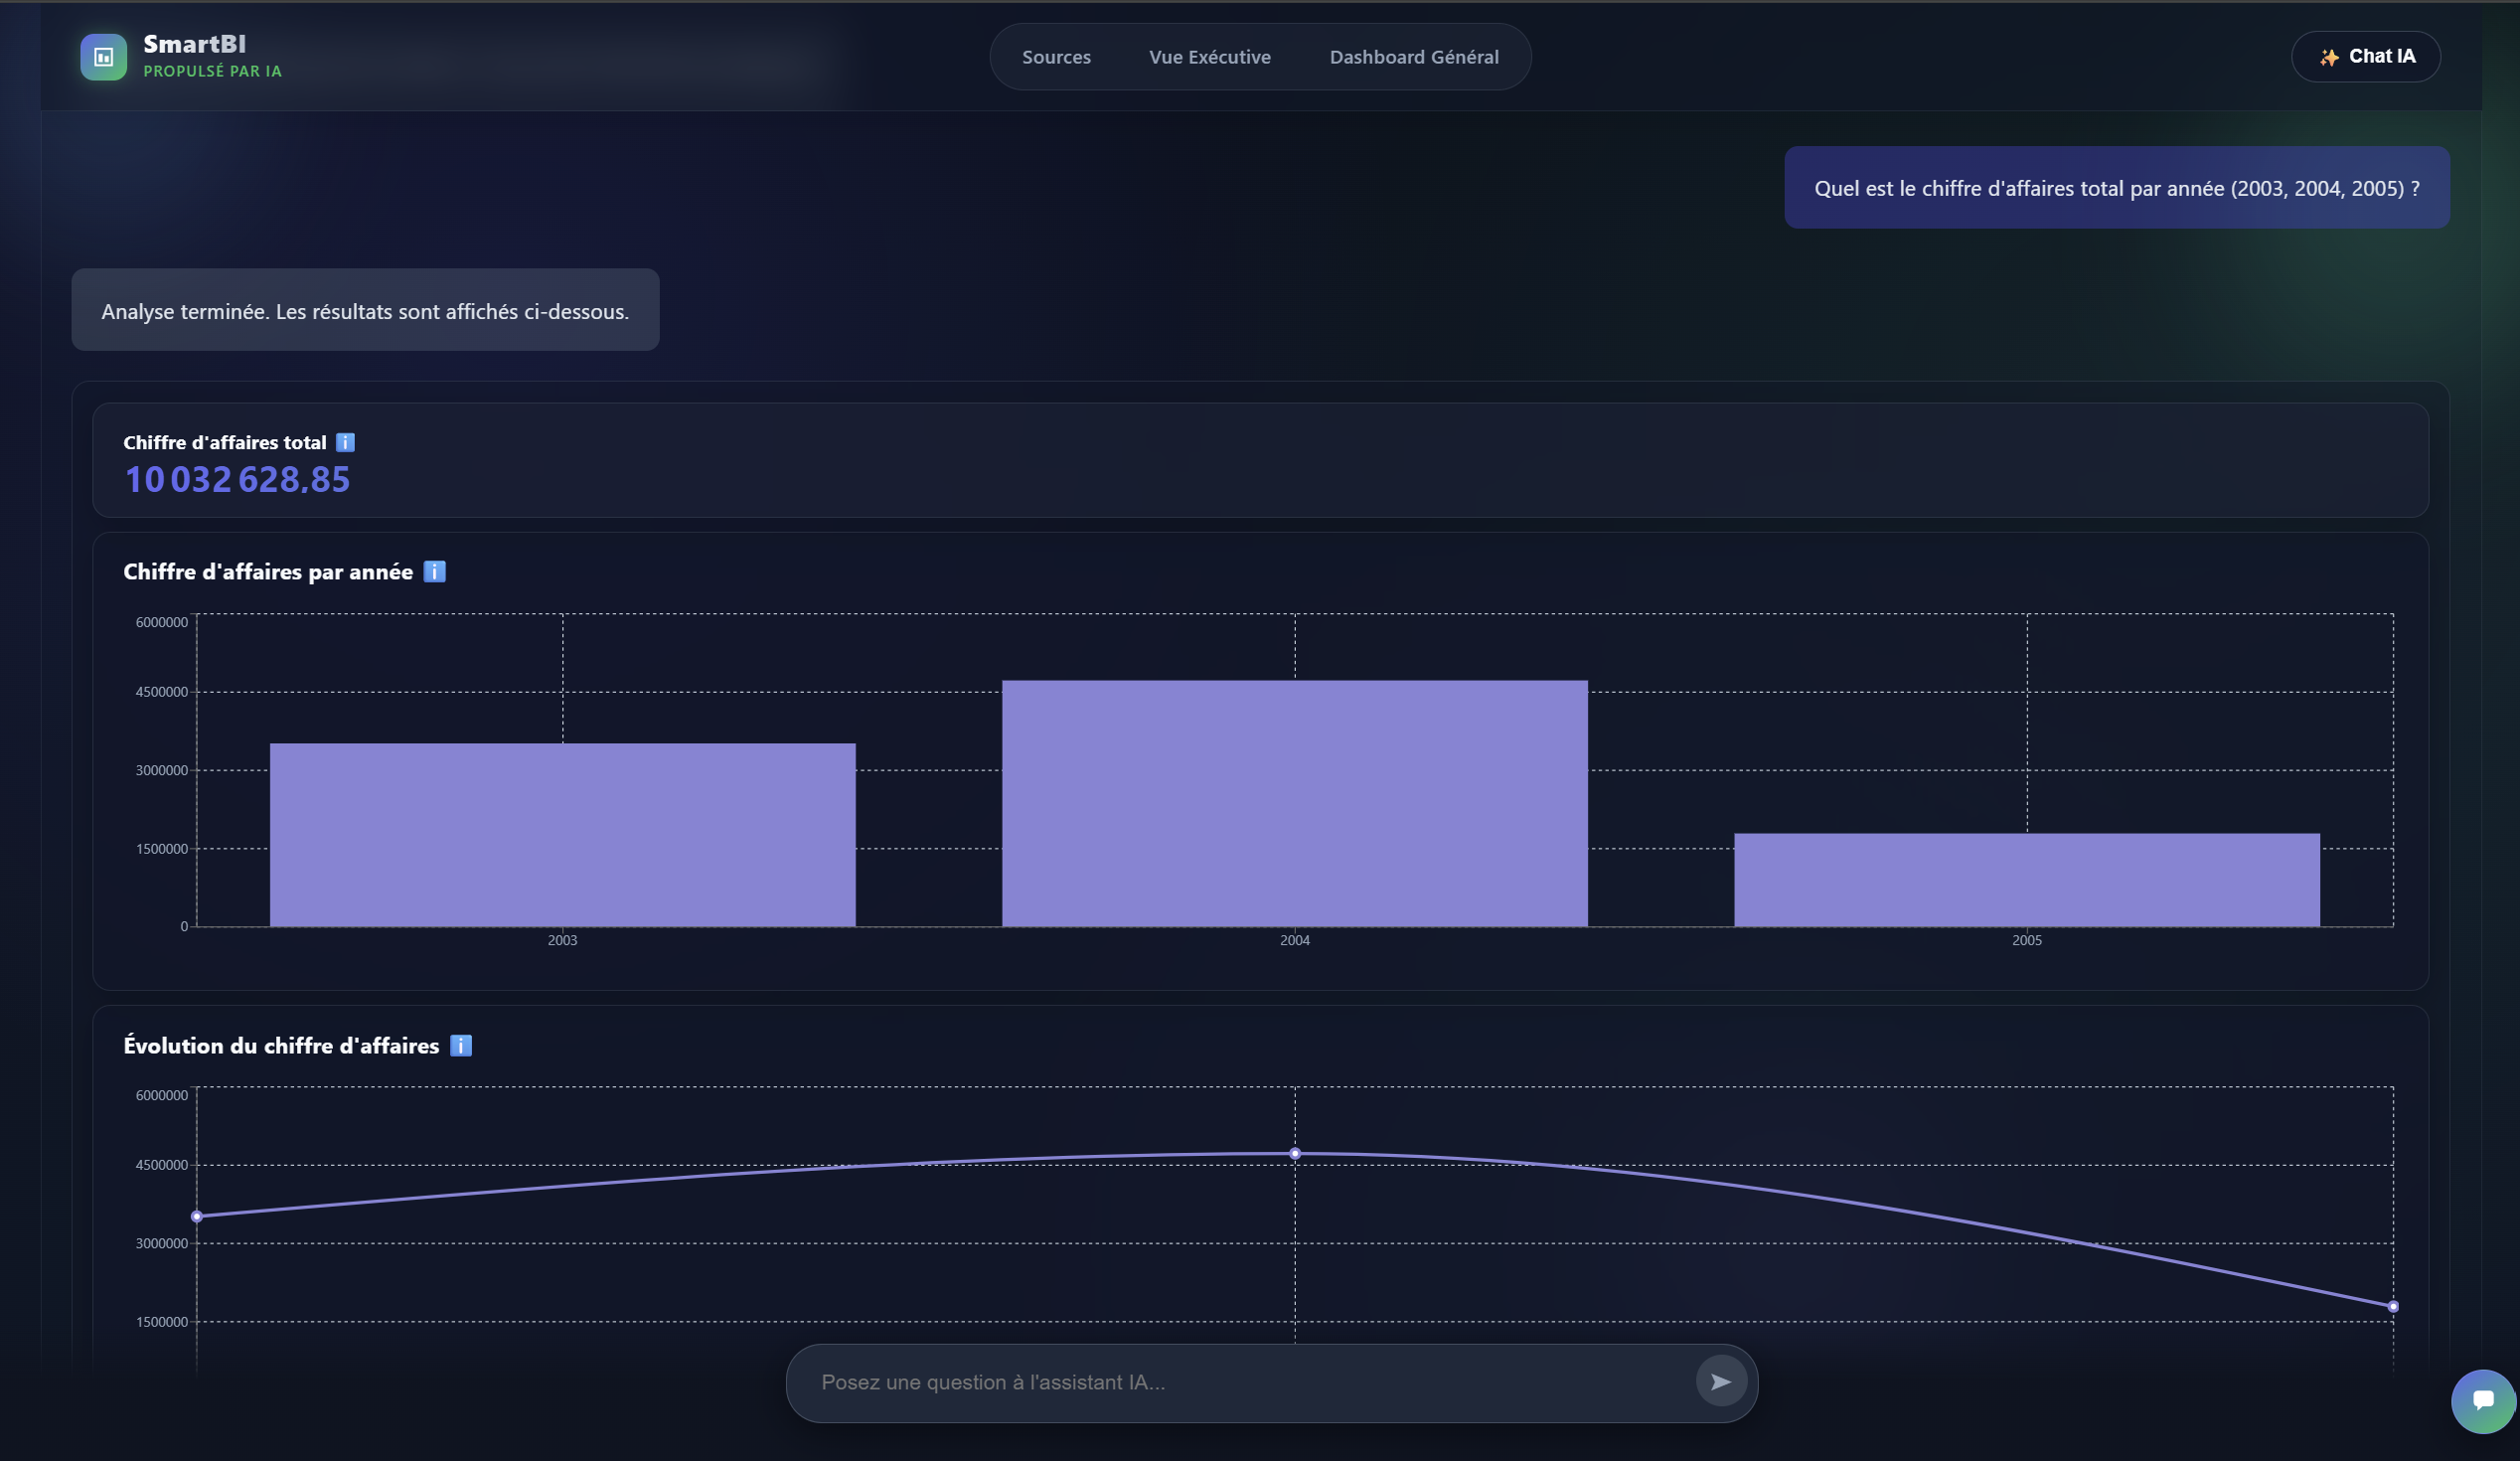
\includegraphics[width=\textwidth]{Smartbi/Screenshot 2026-06-22 181118.png}
\caption{Réponse conversationnelle avec graphique}
\label{fig:filtrage}
\end{figure}

\subsection{Scénario 3 : Auto-correction d'une erreur SQL}

Lors de la génération d'une requête, l'agent ingénieur peut produire une requête utilisant une syntaxe incompatible avec SQLite. L'exécution échoue et l'erreur est capturée. Au second essai, le prompt inclut le message d'erreur et l'agent corrige automatiquement sa requête. Ce mécanisme de retry avec feedback assure un taux de succès élevé pour la génération SQL.

\section{Difficultés rencontrées et solutions}

\subsection{Fiabilité de la génération SQL}

La génération de SQL par un LLM présente un taux d'erreur non négligeable, notamment pour les fonctions de date spécifiques à SQLite et les agrégations imbriquées. Le mécanisme de retry avec feedback d'erreur s'est révélé efficace : dans la majorité des cas, la deuxième tentative produit une requête correcte.

\subsection{Latence du pipeline}

L'exécution séquentielle des trois agents induit une latence cumulée de 30 à 60 secondes. Le streaming NDJSON pour l'upload atténue cette latence perçue en fournissant un retour visuel continu. Pour le mode conversationnel, un indicateur de chargement informe l'utilisateur.

\subsection{Qualité des visualisations}

La pertinence des visualisations dépend de la capacité du LLM à choisir le type de graphique approprié. Des instructions explicites dans les prompts du designer (PieChart pour les distributions, LineChart pour les séries temporelles, etc.) améliorent significativement les résultats.

\section{Synthèse}

La phase de réalisation a abouti à un prototype fonctionnel complet. SmartBI est capable de recevoir un fichier de données, de l'analyser automatiquement via un pipeline multi-agents, de générer des tableaux de bord interactifs et de répondre à des questions en langage naturel. Les mécanismes d'auto-correction, de streaming de progression et de persistance de l'état contribuent à une expérience utilisateur fluide et professionnelle.

%==============================================================================
% CONCLUSION GÉNÉRALE
%==============================================================================
\chapter*{Conclusion Générale}
\addcontentsline{toc}{chapter}{Conclusion Générale}

Ce projet de fin d'année nous a permis de concevoir et de réaliser \textbf{SmartBI}, une plateforme de Business Intelligence pilotée par des agents d'intelligence artificielle utilisant LangGraph et des modèles de langage locaux. L'objectif central était de démontrer qu'il est possible de démocratiser l'accès à l'analyse de données en combinant les capacités de compréhension du langage naturel des LLM avec une architecture multi-agents structurée et résiliente.

Au terme de ce travail, les principaux résultats obtenus sont les suivants. Un pipeline multi-agents fonctionnel a été implémenté, orchestrant la collaboration entre un analyste métier, un ingénieur de données et un designer, avec un mécanisme d'auto-correction des erreurs SQL permettant une fiabilité accrue. Une interface utilisateur moderne et réactive a été développée, offrant un chargement de données par glisser-déposer avec suivi de progression en temps réel, des tableaux de bord interactifs avec filtrage temporel, et une interface de dialogue en langage naturel. L'exécution locale des modèles de langage via Ollama garantit la souveraineté des données, répondant à une préoccupation croissante dans le contexte de la protection des données sensibles.

Sur le plan personnel et professionnel, ce projet nous a permis de développer des compétences approfondies dans plusieurs domaines : l'architecture multi-agents et l'orchestration de workflows IA avec LangGraph, le développement d'applications web full-stack avec Django et React, l'ingénierie des prompts pour des tâches spécialisées (génération SQL, design de dashboards), et la gestion de projet itérative dans un contexte de recherche appliquée.

Plusieurs perspectives d'amélioration et d'extension se dessinent pour les travaux futurs :

\begin{itemize}[leftmargin=2cm]
    \item \textbf{Authentification multi-utilisateurs} : ajout d'un système d'authentification avec gestion de profils pour supporter des environnements collaboratifs en entreprise.
    \item \textbf{Sources de données distantes} : connexion à des bases de données PostgreSQL, MySQL et à des API REST pour étendre le champ d'application au-delà des fichiers locaux.
    \item \textbf{Streaming conversationnel} : implémentation du streaming pour les réponses du mode chat afin de réduire la latence perçue et améliorer l'expérience utilisateur.
    \item \textbf{Mémoire conversationnelle} : intégration d'un mécanisme de mémoire permettant au système de maintenir un contexte d'analyse sur plusieurs tours de dialogue, facilitant les analyses itératives et approfondies.
    \item \textbf{Évaluation systématique} : mise en place de métriques de pertinence des dashboards générés et réalisation de tests utilisateurs pour valider scientifiquement l'approche.
\end{itemize}

En conclusion, ce projet démontre le potentiel des architectures multi-agents basées sur des LLM locaux pour transformer le paysage de la Business Intelligence. En réduisant la barrière technique entre les données et les décideurs, SmartBI ouvre la voie à une nouvelle génération d'outils décisionnels véritablement intelligents et accessibles.

%==============================================================================
% BIBLIOGRAPHIE
%==============================================================================
\begin{thebibliography}{99}
\addcontentsline{toc}{chapter}{Bibliographie}

\bibitem{langgraph}
LangChain, \textit{LangGraph: Build stateful, multi-actor applications with LLMs}, \url{https://langchain-ai.github.io/langgraph/}, 2024.

\bibitem{langchain}
H. Chase, \textit{LangChain: Building applications with LLMs through composability}, \url{https://python.langchain.com/}, 2023.

\bibitem{ollama}
Ollama, \textit{Get up and running with large language models locally}, \url{https://ollama.com/}, 2024.

\bibitem{react}
Meta Platforms, \textit{React -- The library for web and native user interfaces}, \url{https://react.dev/}, 2024.

\bibitem{django}
Django Software Foundation, \textit{Django -- The web framework for perfectionists with deadlines}, \url{https://www.djangoproject.com/}, 2024.

\bibitem{recharts}
Recharts, \textit{A composable charting library built on React components}, \url{https://recharts.org/}, 2024.

\bibitem{qwen}
Alibaba Cloud, \textit{Qwen: Large language model series from Alibaba}, \url{https://github.com/QwenLM/Qwen}, 2024.

\bibitem{generativebi}
Gartner, \textit{Augmented Analytics and Generative BI: The Future of Data Analytics}, Gartner Research, 2024.

\bibitem{pandas}
W. McKinney, \textit{Data Structures for Statistical Computing in Python}, Proceedings of the 9th Python in Science Conference, 2010.

\bibitem{sqlite}
D. R. Hipp, \textit{SQLite: The Database Engine That Powers the World}, \url{https://www.sqlite.org/}, 2024.

\bibitem{multigent}
S. Yao et al., \textit{ReAct: Synergizing Reasoning and Acting in Language Models}, ICLR 2023.

\bibitem{text2sql}
J. Li et al., \textit{DIN-SQL: Decomposed In-Context Learning of Text-to-SQL with Self-Correction}, NeurIPS 2023.

\end{thebibliography}

% \include{chapitres/bibliographie}
% \include{chapitres/annexes}


\end{document}
